%% LyX 2.4.3 created this file.  For more info, see https://www.lyx.org/.
%% Do not edit unless you really know what you are doing.
\documentclass[journal,article,submit,pdftex,moreauthors]{Definitions/mdpi}
\usepackage{textcomp}
\usepackage[utf8]{inputenc}
\usepackage{float}
\usepackage{varwidth}
\usepackage{amsmath}
\usepackage{graphicx}
\usepackage{rotfloat}

\makeatletter

%%%%%%%%%%%%%%%%%%%%%%%%%%%%%% LyX specific LaTeX commands.

\Title{Healing Intelligence: A Bio-Inspired Metaheuristic optimization method
Using Recovery Dynamics}

\TitleCitation{Healing Intelligence: A Bio-Inspired Metaheuristic optimization method
Using Recovery Dynamicss}

\Author{Vasileios Charilogis$^{1}$, Ioannis G. Tsoulos$^{2,*}$ }

\AuthorNames{Vasileios Charilogis, Ioannis G. Tsoulos}

\AuthorCitation{Charilogis, V.; Tsoulos, I.G.}


\address{$^{1}$\quad{}Department of Informatics and Telecommunications,
University of Ioannina, 47150 Kostaki Artas, Greece; v.charilog@uoi.gr\\
$^{2}$\quad{}Department of Informatics and Telecommunications, University
of Ioannina, 47150 Kostaki Artas, Greece; itsoulos@uoi.gr}


\corres{Correspondence: itsoulos@uoi.gr}


\abstract{BioHealing Optimization (BHO) is a bio-inspired metaheuristic optimization
algorithm that emulates the biological process of injury and recovery.
Its operation follows a cyclical mechanism comprising three main stages:
an optional recombination phase, an injury phase, and a healing phase.
During recombination, elements from the best-known solution are combined
with differences drawn from other population members, producing candidate
solutions that inherit beneficial traits while maintaining diversity.
The injury phase applies stochastic perturbations to selected dimensions
of solutions, using either Gaussian-like distributions or heavy-tailed
variations, thereby promoting exploration of new regions in the search
space. In the healing phase, the altered dimensions are guided gradually
toward the current best solution, mimicking the progressive restoration
of function observed in biological tissues. These core mechanisms
are enhanced through adaptive strategies, including dynamic adjustment
of injury intensity and probability, a “scar mapping” system that
stores directional trends, focus on dimensions of higher relevance,
and the introduction of high-intensity disturbance phases to overcome
stagnation. The combination of these elements results in a self-regulating
search process that maintains a balance between exploration and exploitation,
enabling effective performance on challenging continuous optimization
problems.}


\keyword{Bio-inspired Algorithms; Metaheuristics; Regenerative Computing;
Wound Healing; Evolutionary Algorithms; Global Optimization; Mutation
Strategies; }

\newcommand*\LyXZeroWidthSpace{\hspace{0pt}}
\DeclareTextSymbolDefault{\textquotedbl}{T1}
%% Because html converters don't know tabularnewline
\providecommand{\tabularnewline}{\\}
%% Variable width box for table cells
\newenvironment{cellvarwidth}[1][t]
    {\begin{varwidth}[#1]{\linewidth}}
    {\@finalstrut\@arstrutbox\end{varwidth}}
\floatstyle{ruled}
\newfloat{algorithm}{tbp}{loa}
\providecommand{\algorithmname}{Algorithm}
\floatname{algorithm}{\protect\algorithmname}

%%%%%%%%%%%%%%%%%%%%%%%%%%%%%% User specified LaTeX commands.
\usepackage{rotating}

%  LaTeX support: latex@mdpi.com 
%  For support, please attach all files needed for compiling as well as the log file, and specify your operating system, LaTeX version, and LaTeX editor.

%=================================================================


% For posting an early version of this manuscript as a preprint, you may use "preprints" as the journal and change "submit" to "accept". The document class line would be, e.g., \documentclass[preprints,article,accept,moreauthors,pdftex]{mdpi}. This is especially recommended for submission to arXiv, where line numbers should be removed before posting. For preprints.org, the editorial staff will make this change immediately prior to posting.

%--------------------
% Class Options:
%--------------------
%----------
% journal
%----------
% Choose between the following MDPI journals:
% acoustics, actuators, addictions, admsci, adolescents, aerospace, agriculture, agriengineering, agronomy, ai, algorithms, allergies, alloys, analytica, animals, antibiotics, antibodies, antioxidants, applbiosci, appliedchem, appliedmath, applmech, applmicrobiol, applnano, applsci, aquacj, architecture, arts, asc, asi, astronomy, atmosphere, atoms, audiolres, automation, axioms, bacteria, batteries, bdcc, behavsci, beverages, biochem, bioengineering, biologics, biology, biomass, biomechanics, biomed, biomedicines, biomedinformatics, biomimetics, biomolecules, biophysica, biosensors, biotech, birds, bloods, blsf, brainsci, breath, buildings, businesses, cancers, carbon, cardiogenetics, catalysts, cells, ceramics, challenges, chemengineering, chemistry, chemosensors, chemproc, children, chips, cimb, civileng, cleantechnol, climate, clinpract, clockssleep, cmd, coasts, coatings, colloids, colorants, commodities, compounds, computation, computers, condensedmatter, conservation, constrmater, cosmetics, covid, crops, cryptography, crystals, csmf, ctn, curroncol, currophthalmol, cyber, dairy, data, dentistry, dermato, dermatopathology, designs, diabetology, diagnostics, dietetics, digital, disabilities, diseases, diversity, dna, drones, dynamics, earth, ebj, ecologies, econometrics, economies, education, ejihpe, electricity, electrochem, electronicmat, electronics, encyclopedia, endocrines, energies, eng, engproc, ent, entomology, entropy, environments, environsciproc, epidemiologia, epigenomes, est, fermentation, fibers, fintech, fire, fishes, fluids, foods, forecasting, forensicsci, forests, foundations, fractalfract, fuels, futureinternet, futureparasites, futurepharmacol, futurephys, futuretransp, galaxies, games, gases, gastroent, gastrointestdisord, gels, genealogy, genes, geographies, geohazards, geomatics, geosciences, geotechnics, geriatrics, hazardousmatters, healthcare, hearts, hemato, heritage, highthroughput, histories, horticulturae, humanities, humans, hydrobiology, hydrogen, hydrology, hygiene, idr, ijerph, ijfs, ijgi, ijms, ijns, ijtm, ijtpp, immuno, informatics, information, infrastructures, inorganics, insects, instruments, inventions, iot, j, jal, jcdd, jcm, jcp, jcs, jdb, jeta, jfb, jfmk, jimaging, jintelligence, jlpea, jmmp, jmp, jmse, jne, jnt, jof, joitmc, jor, journalmedia, jox, jpm, jrfm, jsan, jtaer, jzbg, kidney, kidneydial, knowledge, land, languages, laws, life, liquids, literature, livers, logics, logistics, lubricants, lymphatics, machines, macromol, magnetism, magnetochemistry, make, marinedrugs, materials, materproc, mathematics, mca, measurements, medicina, medicines, medsci, membranes, merits, metabolites, metals, meteorology, methane, metrology, micro, microarrays, microbiolres, micromachines, microorganisms, microplastics, minerals, mining, modelling, molbank, molecules, mps, msf, mti, muscles, nanoenergyadv, nanomanufacturing, nanomaterials, ncrna, network, neuroglia, neurolint, neurosci, nitrogen, notspecified, nri, nursrep, nutraceuticals, nutrients, obesities, oceans, ohbm, onco, oncopathology, optics, oral, organics, organoids, osteology, oxygen, parasites, parasitologia, particles, pathogens, pathophysiology, pediatrrep, pharmaceuticals, pharmaceutics, pharmacoepidemiology, pharmacy, philosophies, photochem, photonics, phycology, physchem, physics, physiologia, plants, plasma, pollutants, polymers, polysaccharides, poultry, powders, preprints, proceedings, processes, prosthesis, proteomes, psf, psych, psychiatryint, psychoactives, publications, quantumrep, quaternary, qubs, radiation, reactions, recycling, regeneration, religions, remotesensing, reports, reprodmed, resources, rheumato, risks, robotics, ruminants, safety, sci, scipharm, seeds, sensors, separations, sexes, signals, sinusitis, skins, smartcities, sna, societies, socsci, software, soilsystems, solar, solids, sports, standards, stats, stresses, surfaces, surgeries, suschem, sustainability, symmetry, synbio, systems, taxonomy, technologies, telecom, test, textiles, thalassrep, thermo, tomography, tourismhosp, toxics, toxins, transplantology, transportation, traumacare, traumas, tropicalmed, universe, urbansci, uro, vaccines, vehicles, venereology, vetsci, vibration, viruses, vision, waste, water, wem, wevj, wind, women, world, youth, zoonoticdis 

%---------
% article
%---------
% The default type of manuscript is "article", but can be replaced by: 
% abstract, addendum, article, book, bookreview, briefreport, casereport, comment, commentary, communication, conferenceproceedings, correction, conferencereport, entry, expressionofconcern, extendedabstract, datadescriptor, editorial, essay, erratum, hypothesis, interestingimage, obituary, opinion, projectreport, reply, retraction, review, perspective, protocol, shortnote, studyprotocol, systematicreview, supfile, technicalnote, viewpoint, guidelines, registeredreport, tutorial
% supfile = supplementary materials

%----------
% submit
%----------
% The class option "submit" will be changed to "accept" by the Editorial Office when the paper is accepted. This will only make changes to the frontpage (e.g., the logo of the journal will get visible), the headings, and the copyright information. Also, line numbering will be removed. Journal info and pagination for accepted papers will also be assigned by the Editorial Office.

%------------------
% moreauthors
%------------------
% If there is only one author the class option oneauthor should be used. Otherwise use the class option moreauthors.

%---------
% pdftex
%---------
% The option pdftex is for use with pdfLaTeX. If eps figures are used, remove the option pdftex and use LaTeX and dvi2pdf.

%=================================================================
% MDPI internal commands - do not modify
\firstpage{1} 
 
\setcounter{page}{\@firstpage} 

\pubvolume{1}
\issuenum{1}
\articlenumber{0}
\pubyear{2024}
\copyrightyear{2024}
%\externaleditor{Academic Editor: Firstname Lastname} % For journal Automation, please change Academic Editor to "Communicated by"
\datereceived{}
\daterevised{ } % Comment out if no revised date
\dateaccepted{}
\datepublished{}
%\datecorrected{} % Corrected papers include a "Corrected: XXX" date in the original paper.
%\dateretracted{} % Corrected papers include a "Retracted: XXX" date in the original paper.
\hreflink{https://doi.org/} % If needed use \linebreak
%\doinum{}
%------------------------------------------------------------------
% The following line should be uncommented if the LaTeX file is uploaded to arXiv.org
%\pdfoutput=1

%=================================================================
% Add packages and commands here. The following packages are loaded in our class file: fontenc, inputenc, calc, indentfirst, fancyhdr, graphicx, epstopdf, lastpage, ifthen, lineno, float, amsmath, setspace, enumitem, mathpazo, booktabs, titlesec, etoolbox, tabto, xcolor, soul, multirow, microtype, tikz, totcount, changepage, attrib, upgreek, cleveref, amsthm, hyphenat, natbib, hyperref, footmisc, url, geometry, newfloat, caption

%=================================================================
%% Please use the following mathematics environments: Theorem, Lemma, Corollary, Proposition, Characterization, Property, Problem, Example, ExamplesandDefinitions, Hypothesis, Remark, Definition, Notation, Assumption
%% For proofs, please use the proof environment (the amsthm package is loaded by the MDPI class).

%=================================================================
% The fields PACS, MSC, and JEL may be left empty or commented out if not applicable
%\PACS{J0101}
%\MSC{}
%\JEL{}

%%%%%%%%%%%%%%%%%%%%%%%%%%%%%%%%%%%%%%%%%%
% Only for the journal Diversity
%\LSID{\url{http://}}

%%%%%%%%%%%%%%%%%%%%%%%%%%%%%%%%%%%%%%%%%%
% Only for the journal Applied Sciences:
%\featuredapplication{Authors are encouraged to provide a concise description of the specific application or a potential application of the work. This section is not mandatory.}
%%%%%%%%%%%%%%%%%%%%%%%%%%%%%%%%%%%%%%%%%%

%%%%%%%%%%%%%%%%%%%%%%%%%%%%%%%%%%%%%%%%%%
% Only for the journal Data:
%\dataset{DOI number or link to the deposited data set in cases where the data set is published or set to be published separately. If the data set is submitted and will be published as a supplement to this paper in the journal Data, this field will be filled by the editors of the journal. In this case, please make sure to submit the data set as a supplement when entering your manuscript into our manuscript editorial system.}

%\datasetlicense{license under which the data set is made available (CC0, CC-BY, CC-BY-SA, CC-BY-NC, etc.)}

%%%%%%%%%%%%%%%%%%%%%%%%%%%%%%%%%%%%%%%%%%
% Only for the journal Toxins
%\keycontribution{The breakthroughs or highlights of the manuscript. Authors can write one or two sentences to describe the most important part of the paper.}

%%%%%%%%%%%%%%%%%%%%%%%%%%%%%%%%%%%%%%%%%%
% Only for the journal Encyclopedia
%\encyclopediadef{Instead of the abstract}
%\entrylink{The Link to this entry published on the encyclopedia platform.}
%%%%%%%%%%%%%%%%%%%%%%%%%%%%%%%%%%%%%%%%%%

%%%%%%%%%%%%%%%%%%%%%%%%%%%%%%%%%%%%%%%%%%
% Only for the journal Advances in Respiratory Medicine
%\addhighlights{yes}
%\renewcommand{\addhighlights}{%

%\noindent This is an obligatory section in “Advances in Respiratory Medicine”, whose goal is to increase the discoverability and readability of the article via search engines and other scholars. Highlights should not be a copy of the abstract, but a simple text allowing the reader to quickly and simplified find out what the article is about and what can be cited from it. Each of these parts should be devoted up to 2~bullet points.\vspace{3pt}\\
%\textbf{What are the main findings?}
% \begin{itemize}[labelsep=2.5mm,topsep=-3pt]
% \item First bullet.
% \item Second bullet.
% \end{itemize}\vspace{3pt}
%\textbf{What is the implication of the main finding?}
% \begin{itemize}[labelsep=2.5mm,topsep=-3pt]
% \item First bullet.
% \item Second bullet.
% \end{itemize}
%}
%%%%%%%%%%%%%%%%%%%%%%%%%%%%%%%%%%%%%%%%%%
% Added by lyx2lyx
\usepackage{array}

\makeatother

\begin{document}
\maketitle

\section{Introduction}

Global optimization refers to the task of identifying the global minimum
of a real-valued, continuous objective function $f(x)$ , where the
variable $x$ belongs to a predefined, bounded search space $S\subset\mathbb{R}^{n}$.
The goal is to determine the point $x^{*}\in S$ such that the function
$f(x)$ achieves its lowest possible value over the entire domain:

\begin{equation}
x^{*}=\mbox{arg}\min_{x\in S}f(x).
\end{equation}
where:
\begin{itemize}
\item $f(x)$: is the objective function to be minimized. This function
can represent a variety of criteria depending on the problem context,
such as cost, loss, error, potential energy, or any other performance
metric.
\item $S$: is the feasible search space, a compact subset of $\mathbb{R}^{n}$,
meaning it is both closed and bounded. Typically, $S$ is defined
as an $n$-dimensional hyperrectangle (also called a box constraint),
given by:
\end{itemize}
\textbf{
\[
S=\left[a_{1},b_{1}\right]\otimes\left[a_{2},b_{2}\right]\otimes\ldots\left[a_{n},b_{n}\right]
\]
}

This denotes that each variable $x_{i}$ is constrained within a finite
interval: $x_{i\LyXZeroWidthSpace}\in[a_{i\LyXZeroWidthSpace},b_{i}\LyXZeroWidthSpace]\text{,for }i=1,2,...,n=\text{1,2,...,}n$.
The Cartesian product of these intervals defines the multidimensional
region where the search for the global optimum takes place.

Optimization is one of the most fundamental and widely applied domains
of computational intelligence, with a vast range of applications in
scientific, technological, and industrial fields. Although classical
optimization techniques can be effective for small- or medium-scale
problems, they often fail to deliver satisfactory results when applied
to complex, nonlinear, and high-dimensional environments, where issues
such as non-convexity, high dimensionality, and the presence of multiple
local optima dominate the search landscape. In this context, recent
years have seen a continuous rise in interest toward metaheuristic
methods, which offer flexible and stochastic search tools capable
of addressing complex optimization problems without requiring derivative
information or assumptions of continuity in the solution space.

Metaheuristic techniques are typically inspired by natural, biological,
social, or physical processes, aiming to simulate powerful mechanisms
for balancing exploration and exploitation within complex search spaces.
Classic examples include Genetic Algorithms (GA) \citep{Holland},
Particle Swarm Optimization (PSO) \citep{Kennedy}, and Ant Colony
Optimization (ACO) \citep{Dorigo}, which have been widely used for
decades. In recent years, however, a multitude of novel metaheuristics
have emerged, motivated by the desire to overcome common limitations
such as premature convergence and weak performance on rugged, multimodal
landscapes \citep{Talbi}. These methods draw inspiration from a broad
range of biological and ecological systems. From the animal kingdom,
algorithms like Artificial Bee Colony (ABC) \citep{Karaboga}, Grey
Wolf Optimizer (GWO) \citep{Mirjalili1}, Whale Optimization Algorithm
(WOA) \citep{Mirjalili2}, Dragonfly Algorithm (DA) \citep{Mirjalili3},
Cuckoo Search (CS) \citep{Yang2}, and Bat Algorithm \citep{Yang3}
emulate foraging, social, or navigation behaviors. Predator--prey-based
algorithms such as Harris Hawks Optimization (HHO) \citep{Heidari}
and Snake Optimizer \citep{Hashim} capture hunting dynamics. Others
derive from insect colonies or swarm intelligence, including Firefly
Algorithm \citep{Yang4}, Glowworm Swarm Optimization (GSO) \citep{Krishnanand},
and Butterfly Optimization \citep{Arora}. Likewise, bacterial or
microbial behaviors inspire algorithms such as Bacterial Foraging
Optimization (BFO) \citep{Passino}, Virus Colony Search \citep{Li1},
and COVIDOA \citep{Al}. Some algorithms are motivated by botanical
and plant behavior, such as the Plant Propagation Algorithm (PPA)
\citep{Salhi}, Invasive Weed Optimization (IWO) \citep{Mehrabian},
and Root Growth Optimizer \citep{Zhou}. Other methods emerge from
natural physical phenomena, including Gravitational Search Algorithm
(GSA) \citep{Rashedi}, Simulated Annealing \citep{Kirkpatrick},
and the Harmony Search algorithm \citep{Geem}. More recently, complex
hybrid and bio-inspired models such as Gorilla Troops Optimization
(GTO) \citep{Sallam}, Reptile Search Algorithm (RSA) \citep{Abualigah2},
Sine Cosine Algorithm (SCA) \citep{Mirjalili4}, and Slime Mould Algorithm
(SMA) \citep{Li} have been introduced. Despite the thematic diversity
and creativity of modern bio-inspired metaheuristic techniques, many
of them continue to face common shortcomings, such as the lack of
truly adaptive dynamics, a static and rigid balance between exploration
and exploitation, and the absence of documented convergence guarantees
\citep{Boussa=0000EFd}.These limitations underline the need for next-generation
algorithms capable of self-regulating their behavior according to
the state of the search, maintaining stability in convergence, and
faithfully reflecting the principles and rhythms of complex biological
processes.

BioHealing Optimization (BHO) is positioned within this scientific
and technological context, drawing inspiration from the regenerative
process of wound healing in living organisms. Wound healing is a natural
function characterized by a delicate balance between disruption and
restoration, aimed at re-establishing homeostasis. BHO translates
this biological principle into the optimization domain, creating a
multi-phase methodology in which each phase has a distinct yet interdependent
role.
\begin{enumerate}
\item \textbf{Injury phase}: Rather than relying on static or simplistic
modifications, BHO applies stochastic disturbances to selected dimensions
of candidate solutions, emulating the initial, uncontrolled nature
of biological injury. These disturbances may follow distributions
that favor either gentler changes or rare, high-impact shifts, with
their intensity dynamically adapted as the search progresses encouraging
broad exploration in the early stages and gradually reducing disruption
near convergence.
\item \textbf{Healing phase}: Subsequently, BHO selectively guides the modified
dimensions toward the best-known solution, in a process that mirrors
the progressive restoration of biological tissues. This movement is
neither mechanical nor fixed the proportion and direction of adjustments
are adapted to the search conditions, maintaining diversity while
also enhancing the exploitation of high-quality solutions.
\item \textbf{Recombination phase}: Optionally, this process is preceded
by an information exchange mechanism inspired by Differential Evolution,
where components of the best solution are combined with differences
from other members of the population. This allows the inheritance
of strong traits while simultaneously introducing variations that
keep the search active.
\end{enumerate}
Previous approaches inspired by healing processes, such as Wound Healing
Based Optimization (WHO) \citep{Chawla} and the Synergistic Fibroblast
Optimization (SFO) \citep{Dhivyaprabha}, while interesting, implement
more macroscopic models or focus primarily on biological analogies
without a clear separation between exploration and exploitation. They
also do not employ adaptive stochastic perturbations or integrate
evolutionary recombination mechanisms.

In contrast, BHO combines stochastic disruption, guided restoration,
and evolutionary recombination into a single, flexible architecture
that transitions smoothly and self-regulates from exploration to exploitation.
It further incorporates innovations such as dynamic adjustment of
injury and healing probabilities and intensities, a “scar mapping”
system that retains memory of improvement directions, focus on critical
dimensions, and the introduction of high-intensity disturbance phases
to overcome stagnation. Together, these elements form a methodological
proposal that is fundamentally distinct from existing approaches and
offers enhanced robustness and performance in demanding, high-dimensional
optimization problems.

The rest of the paper is organized as follows:

The remainder of the paper is organized as follows: Section \ref{subsec:sec:Method}
presents BHO. Subsection \ref{subsec:The-CorePseudo} provides the
core pseudocode, and Subsection \ref{subsec:=00039Cechanisms} details
how the adaptive mechanisms are integrated into the main loop. Section
\ref{sec:Results} describes the experimental protocol and benchmark
suite, Subsection \ref{subsec:benchmarkFunctions} lists the test
functions, and Subsection \ref{subsec:experimentalResults} reports
and analyzes the outcomes. Finally, Section 4 presents the conclusions,
and Section 5 outlines avenues for future work.

\section{The BioHealing Optimizer algorithm \label{subsec:sec:Method}}

\subsection{The basic body of the BioHealing Optimizer pseudocode\label{subsec:The-CorePseudo}}

The overall algorithm of the method follows:
\begin{algorithm}[H]
\caption{The basic body of the BioHealing Optimizer pseudocode\label{alg:basicPseudocode}}

{\footnotesize Input:}{\footnotesize\par}

{\footnotesize\quad $f$: objective function to minimize}{\footnotesize\par}

{\footnotesize\quad $dim$: problem dimensionality}{\footnotesize\par}

{\footnotesize\quad $NP$: population size}{\footnotesize\par}

{\footnotesize\quad $iter_{max}$: maximum number of iterations}{\footnotesize\par}

{\footnotesize\quad $FE_{max}$: maximum number of Function Evaluations}{\footnotesize\par}

{\footnotesize\quad $lower$, $upper$: bounds for each variable}{\footnotesize\par}

{\footnotesize Params:}{\footnotesize\par}

{\footnotesize\quad $w_{s0}$ : initial wound intensity}{\footnotesize\par}

{\footnotesize\quad $w_{p}$ : probability of wounding per dimension}{\footnotesize\par}

{\footnotesize\quad $h_{r}$ : probability of healing per dimension}{\footnotesize\par}

{\footnotesize\quad $r_{p}$ : probability of recombination with the
best solution}{\footnotesize\par}

{\footnotesize\quad $F$ : differential weight scaling factor in recombination}{\footnotesize\par}

{\footnotesize\quad $CR$ : crossover probability in recombination}{\footnotesize\par}

{\footnotesize Output:}{\footnotesize\par}

{\footnotesize\quad $x_{best}$: the best solution found}{\footnotesize\par}

{\footnotesize\quad $f_{best}$: the value of $f$ at best solution}{\footnotesize\par}

{\footnotesize Initialization:}{\footnotesize\par}

{\footnotesize 01 for $i$=1..$NP$:}{\footnotesize\par}

{\footnotesize 02}{\scriptsize{} \hspace{0.5cm}}{\footnotesize{} for $j$=1..$dim$:}{\footnotesize\par}

{\footnotesize 03}{\scriptsize{} \hspace{0.5cm}\hspace{0.5cm}}{\footnotesize$x_{i,j}~U(lower_{j},upper_{j})$}{\footnotesize\par}

{\footnotesize 04}{\scriptsize{} \hspace{0.5cm}}{\footnotesize$fit_{i}=f(x_{i})$}{\footnotesize\par}

{\footnotesize 05 $x_{best}$, $f_{best}$ = argmin($fit_{i}$)}{\footnotesize\par}

{\footnotesize 06 $iter$ = 0}{\footnotesize\par}

{\footnotesize Main loop:}{\footnotesize\par}

{\footnotesize 07 while $iter$ \textless{} $iter_{max}$ or $FE$
\textless{} $FE_{max}$}{\footnotesize\par}

{\footnotesize 08}{\scriptsize{} \hspace{0.5cm}}{\footnotesize$iter$
= $iter$ + 1}{\footnotesize\par}

{\footnotesize 09}{\scriptsize{} \hspace{0.5cm}}{\footnotesize$elite$
= argmin($fit_{i}$)}{\footnotesize\par}

{\footnotesize 10}{\scriptsize{} \hspace{0.5cm}}{\footnotesize$x_{best}$
= $x_{elite}$, fbest = $fit_{elite}$}{\footnotesize\par}

{\footnotesize 11}{\scriptsize{} \hspace{0.5cm}}{\footnotesize$w_{s}$
= max(0.05$\cdot w_{s0}$, $w_{s0}\cdot$(1 - $\frac{iter}{iter_{max}}$))}{\footnotesize\par}

{\footnotesize 12}{\scriptsize{} \hspace{0.5cm}}{\footnotesize for $i$=1..NP:}{\footnotesize\par}

{\footnotesize 13}{\scriptsize{} \hspace{0.5cm}\hspace{0.5cm}}{\footnotesize if
$i$ = $elite$: continue}{\footnotesize\par}

{\footnotesize 14}{\scriptsize{} \hspace{0.5cm}\hspace{0.5cm}}{\footnotesize$x_{old}$
= $x_{i}$, $f_{old}$ = $fit_{i}$}{\footnotesize\par}

{\footnotesize 15}{\scriptsize{} \hspace{0.5cm}\hspace{0.5cm}}{\footnotesize if
$U(0,1)$ \textless{} $r_{p}$:}{\footnotesize\par}

{\footnotesize 16}{\scriptsize{} \hspace{0.5cm}\hspace{0.5cm}\hspace{0.5cm}}{\footnotesize choose
$r_{1}\neq i$, $r_{2}\neq i$, $r_{2}\neq r_{1}$}{\footnotesize\par}

{\footnotesize 17}{\scriptsize{} \hspace{0.5cm}\hspace{0.5cm}\hspace{0.5cm}}{\footnotesize$j_{r}$
= randInt(1,$dim$)}{\footnotesize\par}

{\footnotesize 18}{\scriptsize{} \hspace{0.5cm}\hspace{0.5cm}\hspace{0.5cm}}{\footnotesize for
$j$=1..$dim$:}{\footnotesize\par}

{\footnotesize 19}{\scriptsize{} \hspace{0.5cm}\hspace{0.5cm}\hspace{0.5cm}\hspace{0.5cm}}{\footnotesize if
$U(0,1)$ \textless{} $CR$ or $j$ = $j_{r}$:}{\footnotesize\par}

{\footnotesize 20}{\scriptsize\hspace{0.5cm}\hspace{0.5cm}\hspace{0.5cm}\hspace{0.5cm}\hspace{0.5cm}}{\footnotesize$v$
= $x_{best,j}$ + $F\cdot$($x_{r1,j}$ - $x_{r2,j}$)}{\footnotesize\par}

{\footnotesize 21}{\scriptsize\hspace{0.5cm}\hspace{0.5cm}\hspace{0.5cm}\hspace{0.5cm}\hspace{0.5cm}}{\footnotesize$x_{i,j}$=
clamp($v$, $lower_{j}$, $upper_{j}$)}{\footnotesize\par}

{\footnotesize 22}{\scriptsize\hspace{0.5cm}\hspace{0.5cm}}{\footnotesize for
$j$=1..$dim$:}{\footnotesize\par}

{\footnotesize 23}{\scriptsize\hspace{0.5cm}\hspace{0.5cm}\hspace{0.5cm}}{\footnotesize if
$U(0,1)$ \textless{} $w_{p}$:}{\footnotesize\par}

{\footnotesize 24}{\scriptsize\hspace{0.5cm}\hspace{0.5cm}\hspace{0.5cm}\hspace{0.5cm}}{\footnotesize$\xi$
= stochasticStep() // $N(0,1)$ or Lévy}{\footnotesize\par}

{\footnotesize 25}{\scriptsize\hspace{0.5cm}\hspace{0.5cm}\hspace{0.5cm}\hspace{0.5cm}}{\footnotesize$d$
= $w_{s}\cdot$ $\xi$ $\cdot$ ($upper_{j}$-$lower_{j}$)}{\footnotesize\par}

{\footnotesize 26}{\scriptsize\hspace{0.5cm}\hspace{0.5cm}\hspace{0.5cm}\hspace{0.5cm}}{\footnotesize$x_{i,j}$
= clamp($x_{i,j}$+ $d$, $lower_{j}$, $upper_{j}$)}{\footnotesize\par}

{\footnotesize 27}{\scriptsize\hspace{0.5cm}\hspace{0.5cm}}{\footnotesize$a$
=healStep($hr$)}{\footnotesize\par}

{\footnotesize 28}{\scriptsize\hspace{0.5cm}\hspace{0.5cm}}{\footnotesize for
$j$=1..$dim$:}{\footnotesize\par}

{\footnotesize 29}{\scriptsize\hspace{0.5cm}\hspace{0.5cm}\hspace{0.5cm}}{\footnotesize{}
if $U(0,1)$ \textless{} $h_{r}$:}{\footnotesize\par}

{\footnotesize 30}{\scriptsize\hspace{0.5cm}\hspace{0.5cm}\hspace{0.5cm}\hspace{0.5cm}}{\footnotesize{}
$x_{i,j}$ = clamp($x_{i,j}$ + a($x_{best_{j}}$-$x_{i,j}$), $lower_{j}$,
$upper_{j}$)}{\footnotesize\par}

{\footnotesize 31}{\scriptsize\hspace{0.5cm}\hspace{0.5cm}}{\footnotesize$f_{new}$
= f($x_{i}$)}{\footnotesize\par}

{\footnotesize 32}{\scriptsize\hspace{0.5cm}\hspace{0.5cm}}{\footnotesize if
$f_{new}$ \textless{} $f_{old}$:}{\footnotesize\par}

{\footnotesize 33}{\scriptsize\hspace{0.5cm}\hspace{0.5cm}\hspace{0.5cm}}{\footnotesize$fit_{i}$
= $f_{new}$}{\footnotesize\par}

{\footnotesize 34}{\scriptsize\hspace{0.5cm}\hspace{0.5cm}\hspace{0.5cm}}{\footnotesize if
$f_{new}$ \textless{} $f_{best}$:}{\footnotesize\par}

{\footnotesize 35}{\scriptsize\hspace{0.5cm}\hspace{0.5cm}\hspace{0.5cm}\hspace{0.5cm}}{\footnotesize$f_{best}$
= $f_{new}$ , $x_{best}$ = $x_{i}$}{\footnotesize\par}

{\footnotesize 36}{\scriptsize\hspace{0.5cm}\hspace{0.5cm}\hspace{0.5cm}}{\footnotesize else:}{\footnotesize\par}

{\footnotesize 37}{\scriptsize\hspace{0.5cm}\hspace{0.5cm}\hspace{0.5cm}\hspace{0.5cm}}{\footnotesize$x_{i}$
= $x_{old}$, $fit_{i}$ = $f_{old}$}{\footnotesize\par}

{\footnotesize 38 return $x_{best}$, $f_{best}$}{\footnotesize\par}
\end{algorithm}

The core loop of the BHO maintains a population of candidate solutions
within box constraints and repeatedly balances broad exploration with
guided exploitation. It begins by sampling each vector uniformly within
the per-dimension bounds, evaluating all candidates, and designating
the incumbent best. At every iteration, the current elite is identified
and the wound intensity follows a monotone decay schedule so that
early updates encourage wide exploration while later ones stabilize
around promising regions. For each non-elite individual, an optional
Differential Evolution recombination (best/1, bin) may combine the
incumbent best with a scaled difference of two distinct peers all
values are kept feasible through clamping to the bounds. The injury
phase then applies a per-dimension stochastic disturbance with a specified
probability, using either Gaussian noise or a Lévy-tailed step produced
by a generic stochasticStep() procedure and scaled by the current
wound intensity and the variable range, feasibility is again enforced
by clamping. The healing phase gently attracts modified components
toward the incumbent best with a specified probability, using a step
$a$ = healStep($h_{r}$) that increases with the healing rate and
preserves bounds. The resulting trial is evaluated and accepted greedily
only if it improves the previous fitness whenever an improvement is
accepted, the global best is also updated. The procedure terminates
upon exhausting either the iteration budget or the cap on function
evaluations, and returns the pair ($x_{best}$, $f_{best}$). This
description captures the clean, modular backbone of BHO elite selection,
optional recombination, injury, healing, and greedy replacement while
allowing optional extensions to be integrated without altering the
fundamental methodology.

Below are the core equations of BHO’s three components Injury, Healing,
and Recombination together with the minimal auxiliary relations required
for completeness:

\medskip{}

Notation:
\begin{itemize}
\item $x_{i,j}^{(iter)}$: coordinate $j$ of individual $i$ at iteration
$iter$
\item $[lower_{j},uppe_{j}]$: bounds
\item $x_{best,j}^{(iter)}$: incumbent best
\item clamp($z$, $lower$, $upper$) = min (max($z$, $lower$), $upper$)
\item $U(0,1)$: uniform random in {[}0,1{]}
\end{itemize}
\medskip{}

\begin{enumerate}
\item Injury (stochastic perturbation)

With per-dimension wound probability $w_{p}$ (or adaptive $w_{p,j}$):
\end{enumerate}
\begin{center}
$x_{i,j}^{(iter)}+w_{s}^{(iter)}\,\xi_{i,j}^{(iter)}\,(upper_{j}-lower_{j}),\;lower_{j},\;upper_{j}\Big)$
\par\end{center}

where $\xi_{i,j}^{(t)}=$ stochasticStep() and the wound intensity
$w_{s}^{(t)}$can be scheduled, e.g.,
\begin{center}
$w_{s}^{(iter)}=\max\!\Big(0.05\,w_{s0},\;w_{s0}\big(1-\tfrac{tter}{iter_{\max}}\big)\Big)$
\par\end{center}

Auxiliary (stochastic step definition):
\begin{center}
$\begin{cases}
\mathcal{N}(0,1), & \text{(Gaussian)}\\[4pt]
\text{levyScale}\,\dfrac{u}{|v|^{1/\alpha}},\quad u\sim\mathcal{N}(0,\sigma_{u}^{2}),\;v\sim\mathcal{N}(0,1), & \text{(Lévy/Mantegna)}
\end{cases}$
\par\end{center}

with
\begin{center}
$\sigma_{u}=\left[\frac{\Gamma(1+\alpha)\,\sin\!\big(\pi\alpha/2\big)}{\Gamma\!\big(\tfrac{1+\alpha}{2}\big)\,\alpha\,2^{(\alpha-1)/2}}\right]^{\!1/\alpha}$
\par\end{center}

and an optional global scale levyscale.
\begin{enumerate}
\item Healing (guided move toward $x_{best}$)

With per-dimension healing probability $h_{r}$:
\end{enumerate}
\begin{center}
$x_{i,j}^{(iter,\mathrm{heal})}=clamp\Big(x_{i,j}^{(iter,\mathrm{inj})}+a^{(iter)}\big(x_{best,j}^{(iter)}-x_{i,j}^{(iter,\mathrm{inj})}\big),\;lower_{j},\;upper_{j}\Big)$,
\par\end{center}

\begin{center}
where $a^{(iter)}=\texttt{healStep}\text{(\ensuremath{h_{r}}) (e.g. a simple linear rule}\ensuremath{a^{(iter)}=0.15+0.35\,h_{r}}$,
bounded in $\ensuremath{[0,1)}$)
\par\end{center}
\begin{enumerate}
\item Recombination (DE/best/1/bin)

With probability $r_{p}$ the DE best/1 with binomial crossover is
applied:
\end{enumerate}
\begin{center}
$v=x_{best,j}^{(iter)}+F\big(x_{r1,j}^{(iter)}-x_{r2,j}^{(iter)}\big)$
\par\end{center}

\begin{center}
$C\sim\text{Bernoulli}(\mathrm{CR}),\;\text{enforce }C_{j_{\mathrm{rand}}}=1$
\par\end{center}

\begin{center}
$x_{i,j}^{(iter,\mathrm{rec})}=clamp\Big(C_{j}\,v_{i,j}^{(iter)}+(1-C_{j})\,x_{i,j}^{(iter)},\;lower_{j},\;upper_{j}\Big)$
\par\end{center}
\begin{enumerate}
\item Greedy acceptance

After the phases (in the algorithm’s prescribed order):
\end{enumerate}
\begin{center}
$\text{accept }x_{i}^{\text{new}}\;$$\text{iff}\;f\!\big(x_{i}^{\text{new}}\big)<f\!\big(x_{i}^{\text{old}}\big),$$\quad\text{else revert.}$
\par\end{center}

\subsection{Integration of adaptive mechanisms into the BHO core loop\label{subsec:=00039Cechanisms}}

The integration of the extensions into the BHO core loop follows the
method’s natural flow without altering its backbone. After initialization
and before processing individuals in each iteration, the algorithm
updates stagnation status and configures any exploration bursts at
this point a targeted micro-restart around the incumbent best may
also be triggered when lack of improvement persists. In the same pre-loop
stage, the per-dimension importance scores are decayed and the current
hot set is selected so that subsequent perturbations are preferentially
strengthened where recent gains have been observed.

At the heart of the iteration, immediately before applying stochastic
disturbances, the noise generator is determined: the random step may
use a heavy-tailed Mantegna draw to allow rare long jumps or fall
back to Gaussian noise, depending on settings. The injury phase then
exploits the hot-dimension priorities, the multiplicative burst effects
when RAGE or Hyper-RAGE windows are active, and a mild intensity boost
when early stagnation is detected. The random step is gently biased
toward the recent momentum direction of each coordinate through a
dedicated bias coefficient, while bandage protection can be bypassed
only during bursts so as not to throttle exploration. Immediately
after the standard injuries, a targeted Alpha-Strike may rarely fire
on a few coordinates, scaled by variable ranges and current wound
strength, before control passes to healing.

The healing phase is modulated so that, during bursts, the restorative
rate is temporarily reduced to avoid erasing exploration, followed
by a short cooldown with amplified healing to smooth the return to
stabilization. Optionally, while bursts are active, selected components
may be copied from the incumbent best to inject direction without
sacrificing diversity. Acceptance remains greedy, and only upon true
improvement are the scar-map learning states updated: the per-dimension
wounding probabilities and strengths, momentum, importance scores,
and bandage. These updates feed the next injury cycle, conveying where
and how stronger or more frequent disturbances are worthwhile. When
no improvement occurs, the distance since last best increases and
can re-trigger soft boosts, bursts, or, if needed, micro-restarts
at the beginning of the next iteration. In this way, the mechanisms
are woven into injury, healing, and their transitions, while preserving
the clean core architecture of elite selection, recombination, disturbance,
restoration, and greedy replacement.
\begin{itemize}
\item Scar Map: Momentum \& Bandage

\begin{algorithm}[H]
\caption{Scar Map: Momentum \& Bandage\label{alg:scar}}

Input: $changed_{dims}$ : Which dimensions changed, $towardBest_{j}\in(0,1)$,
$signDir_{j}\in(-1,+1)$$towardBest_{j}$

Params: $scarLR$, $scar_{pmin}$/$scar_{pmax}$, $mom_{decay}$,
$mom_{bias}$, $bandage_{len}$

State: $woundPdim_{j}$, $woundSdim_{j}$, $scarMomentum_{j}$, $bandage_{i,j}$,
$dimScore_{j}$

01 for each $j$ in $changed_{dims}$:

02 {\scriptsize\hspace{0.5cm}}$gP$ = $scarLR$ $\cdot$ (0.5 + 0.5
$\cdot$ $towardBest_{j}$)

03 {\scriptsize\hspace{0.5cm}}$gS$ = $scarLR$ $\cdot$ (0.25 +
0.75 $\cdot$ $towardBest_{j}$)

04 {\scriptsize\hspace{0.5cm}}$woundPdim_{j}$ = clamp($woundPdim_{j}$
+ $gP$, $scar_{pmin}$, $scar_{pmax}$)

05 {\scriptsize\hspace{0.5cm}}$woundSdim_{j}$ = clamp($woundSdim_{j}$
+ $gS$, $scar_{smin}$, $scar_{smax}$)

06 {\scriptsize\hspace{0.5cm}}$scarMomentum_{j}$ = (1 \textminus{}
$mom_{decay}$) $\cdot$ $scarMomentum_{j}$ + $mom_{decay}$$\cdot$
$signDir_{j}$

07 {\scriptsize\hspace{0.5cm}}$dimScore_{j}$ = $dimScore_{j}$ +
improvement\_signal() // e.g. \textbar f\_old \textminus{} f\_new\textbar{}

08 {\scriptsize\hspace{0.5cm}}if $bandage_{len}$ \textgreater{}
0 $bandage_{i,j}$ = $bandage_{len}$ // \textquotedbl freeze\textquotedbl{}
recently improved dimension

09 {\scriptsize\hspace{0.5cm}}if $mom_{bias_{j}}$ = $mom_{bias}$
$\cdot$ sign($scarMomentum_{j}$) 

\end{algorithm}

After each successful acceptance (when the new solution improves the
previous one), Mechanism A updates, per dimension, a “scar map” that
stores two quantities: the future probability of wounding and its
intensity. The update follows the learning rate ($scarLR$) and is
clamped within $scar_{pmin}$/$scar_{pmax}$ and $scar_{smin}$/$scar_{smax}$.
When the accepted change moved toward the current best ($towardBest_{j}$),
the adjustment is strengthened so that dimensions that contributed
to progress are wounded more often and more purposefully later. In
parallel, the momentum term ($scarMomentum_{j}$) keeps a decayed
running sign of recent accepted moves ($signDir_{j}$) using mom\_decay,
allowing the next stochastic step to lean slightly toward the beneficial
direction. The dimension score ($dimScore_{j}$) rises proportionally
to the achieved improvement and later feeds the selection of “hot”
dimensions. Finally, $bandage_{len}$ freezes just-improved dimensions
for a few iterations, protecting the gain from immediate over-disturbance.

Integration with the core loop is straightforward: Mechanism A runs
right after greedy acceptance, only when $f_{new}$ \textless{} $f_{old}$.
In subsequent cycles, the injury phase no longer uses a single wp
but reads the per-dimension $woundPdim_{j}$ and $woundSdim_{j}$
and, where applicable, blends the random disturbance with momentum.
The healing phase remains unchanged, while the bandage temporarily
prevents new wounds on freshly improved dimensions. In this way, the
core stays clean, and the auxiliary structures self-regulate the rate
and targeting of exploration on a per-dimension basis.
\item Hot-Dims Focus (top-K \& boosts for injury)

\begin{algorithm}[H]
\caption{Hot-Dims Focus: Boosting Probability \& Intensity on Top-K Dimensions\label{alg:hot}}

Params:$hotk$, $hotBoost_{p}$, $hotBoost_{s}$, $dim_{decay}$,
$hot$

State : $dimScore_{j}$

01 for $j$= 1..$dim$ $dimScore_{j}$= (1 \textminus{} $dim_{decay}$)
$\cdot$ $dimScore_{j}$

02 $hot$ = topK(dimScore, $hotk$) // steers Injury boosts

03 if $j\in hot$ $p_{base}$ = $p_{base}$ $\cdot hotBoost_{p}$)

04 if $j\in hot$ $scale$ = $scale$ $\cdot hotBoost_{s}$
\end{algorithm}

The Hot-Dims Focus mechanism allocates exploration effort to the coordinates
that have recently contributed to improvement. A mild decay is first
applied to $dimScore_{j}$, ensuring that older gains gradually fade
and more recent signals dominate. From the updated scores, the top
$hotk$ dimensions form the set hot. During the injury phase, if a
coordinate is in hot, its base wounding probability $p_{base}$ is
amplified and the disturbance intensity scale is also increased. This
gently shifts the balance toward components of the search space that
have proven effective, while preserving global diversity across the
remaining dimensions.
\item RAGE \& Hyper-RAGE

\begin{algorithm}[H]
\caption{RAGE / Hyper-RAGE: Explosive exploration under stagnation\label{alg:rage}}

State : $sinceBest$, $rageTimer$, $hyperTimer$

Params: $rageStagnThr$, $rageLen$, $ragePMult$, $rageSMult$, $rageIgnoreBandage$
,

$rage2StagnThr$, $rage2Len$, $rage2PMult$, $rage2SMult$. optional
$copyRate$

01 if $sinceBest$\ensuremath{\ge}$rageStagnThr$ and $rageTimer$=0
$rageTimer$=$rageLen$

02 else if $rageTimer$\textgreater 0 $rageTimer$= $rageTimer$
-1

03 if $sinceBest$\ensuremath{\ge}$rage2_{s}tagn_{t}hr$ and $hyperTimer$=0
$hyperTimer$=$rage2Len$

04 else if $hyperTimer$\textgreater 0 $hyperTimer$ = $hyperTimer$
-1

05 if $rageTimer$\textgreater 0 $pBase$=$pBase$$\cdot ragePMult$
, $scale$=$scale$$\cdot rageSMult$

06 if $hyperTimer$\textgreater 0 $pBase$=0.999 ,$scale$=$scale$$\cdot rage2SMult$

07 if ($rageTimer$\textgreater 0 and $rageIgnorBandage$) or $hyperTimer$\textgreater 0
$bypassBandage$=true

08 if ($rageTimer$\textgreater 0 or $hyperTimer$\textgreater 0)
and $U(0,1)$\textless$copyRate$ $x_{i,j}$ = $x_{best_{j}}$
\end{algorithm}

When the stagnation counter sinceBest exceeds predefined thresholds,
temporary timers for RAGE and Hyper-RAGE ($rageTimer$, $hyperTimer$)
are triggered. While a timer is active, the injury phase is amplified:
in RAGE the base probability and disturbance scale are boosted ($pBase\cdot ragePMult$,
$scale\cdot rageSMult$), whereas in Hyper-RAGE the wounding probability
is driven near certainty and the scale is increased even further (pBase\ensuremath{\approx}1,
scale·rage2SMult). Optionally, bandage protection can be bypassed
($rageIgnoreBandage$) so recently improved coordinates are not shielded,
and components may occasionally be copied from the incumbent best
($copyRate$) to inject direction. The timers count down and, once
expired, the system returns to normal. The aim is to jolt the search
out of local minima during stagnation without altering the algorithm’s
core loop.
\item Lévy-Wounds (Mantegna)

\begin{algorithm}[H]
\caption{Lévy-Wounds (Mantegna): Heavy-tailed jumps for rare long-range moves\label{alg:l=0000E9vy}}

Params: $levyAlpha$, $levyScale$

Precompute: $levySigmaU$

01 levyStep() $u$=$levySigmaU$$\cdot$$N(0,1)$, $v$=$N(0,1)$

02 {\scriptsize\hspace{0.5cm}\hspace{0.5cm}\hspace{0.5cm}}return
$levyScale$ $\cdot$ ($\frac{u}{|v|^{(\frac{1}{levyAlpha})}}$)

03 stochasticStep() return (levyEnabled ? levyStep() : $N(0,1)$)
\end{algorithm}

This mechanism draws heavy-tailed random steps to enable rare, long
jumps that help escape local minima. The $levyAlpha$ parameter controls
tail heaviness (lower values yield more frequent large jumps), while
$levyScale$ sets the step magnitude. The constant $levySigmaU$ is
precomputed (Mantegna scheme), and levyStep() samples two Gaussian
variables to return a Lévy-type increment. The stochasticStep() then
switches between Lévy and standard Gaussian noise, allowing the Injury
phase to mix aggressive exploration with steadier local moves, with
feasibility preserved via clamping.
\item Alpha-Strike

\begin{algorithm}[H]
\caption{Alpha-Strike: Targeted, rare, large jump on a few coordinates\label{alg:alpha}}

Params: $alphaStrikeRate$, $alphaStrikeScale$, $hotK$

State: $bestSample$, $scarMomentum_{j}$

01 if $U(0,1)$\ensuremath{\ge}$alphaStrikeRate$: return

02 $S$ = (hot nonempty ? pick max(1,$\frac{hotK}{2}$) : \{rand $j$\})

03 for $j$ in $S$

04 {\scriptsize\hspace{0.5cm}}step = (1+\textbar stochasticStep()\textbar )$\cdot$$alphaStrikeScale$$\cdot$($upper_{j}$\textminus $lower_{j}$)

05 {\scriptsize\hspace{0.5cm}}$dir$ = choose\{towardBest, momentumSign,
random\}

06 {\scriptsize\hspace{0.5cm}}$x_{j}$ = clamp($x_{j}$ + $ws$$\cdot$$step$$\cdot$$dir$,
$lower_{j}$, $upper_{j}$)
\end{algorithm}

Alpha-Strike triggers with a small probability ($alphaStrikeRate$)
and applies a strong, targeted jump to a small subset of coordinates,
preferably drawn from the current “hot” set ($hotK$). The step magnitude
scales with $alphaStrikeScale$, the variable range, and the current
stochastic term (stochasticStep()), while direction is chosen intelligently:
either toward the incumbent best (towardBest using $bestSample$),
along the momentum sign (momentumSign derived from scarMomentum\_j),
or randomly when diversification is desired. All updates are modulated
by the current wound intensity ws and clamped to the feasible bounds.
The aim is to vault past barriers and local minima swiftly, keeping
the move rare yet highly impactful without disrupting the algorithm’s
core cadence
\item Catastrophic Micro-Reset

\begin{algorithm}[H]
\caption{Catastrophic Micro-Reset: Targeted mini-restart around the incumbent
best\label{alg:catastrophic}}

Params: $catResetThr$, $catResetFrac,$ $catSigma$

State: $sinceBest$, $elite$, $NP$

01 if $sinceBest$\textless$catResetThr$ return

02 $elite$ = $argmin(fit)$

03 $nreset$ = max(1, round($catResetFrac$$\cdot$$NP$))

04 repeat $k$=1..$nreset$ ($i$\ensuremath{\neq}$elite$):

05 for $j$ $cand_{j}$ = clamp($bestSample_{j}$ + $catSigma$$\cdot$($upper_{j}$\textminus $lower_{j}$)$\cdot$$N(0,1)$,
$lower_{j}$, $upper_{j}$)

06 {\scriptsize\hspace{0.5cm}}$f$ = f($cand$)

07 {\scriptsize\hspace{0.5cm}}if $f$\textless{} $fit_{i}$: $x_{i}$=$cand$,
$fit_{i}$=$f$ , updateGlobalBestIfNeeded()
\end{algorithm}

When the search stalls for long enough ($sinceBest$ exceeds $catResetThr$),
a gentle, targeted restart is triggered on a small fraction of the
population. A number of individuals proportional to $catResetFrac$
is selected (always excluding the elite), and for each, a candidate
is sampled near the current $bestSample$ by adding Gaussian noise
scaled by catSigma and each dimension’s range. Values are clamped
to the bounds and evaluated, improvements are accepted greedily and
the global best is updated if necessary. This injects controlled diversity
around promising regions without wiping the population, helping the
search escape local minima quickly with minimal risk.
\item Healing Adjustments \& Cooldown

\begin{algorithm}[H]
\caption{Healing Adjustments \& Cooldown: Modulating healing during bursts
with a smooth post-burst ramp\label{alg:healing}}

Params: $healRageReduce$, $healPostCool$, $cooldownLen$

State: $hr$, $hrate$, $rageTimer$, $hyperTimer$, $cooldown$

01 hrate = $hr$

02 if ($rageTimer$\textgreater 0 or $hyperTime$r\textgreater 0)
$hrate$ = reduce($hrate$, $healRageReduce$)

03 else if $cooldown$\textgreater 0 $hrate$ = increase($hrate$,
$healPostCool$)

04 $alpha$ = healStep($hrate$), applyHealingWith($alpha$)

05 if $burstEnded$ $cooldown$=$cooldownLen$

06 if $cooldown$\textgreater 0 $cooldown$ = $cooldown$-1
\end{algorithm}

This mechanism dynamically tunes the healing rate so exploration remains
effective during bursts and stabilization accelerates immediately
afterward. The base hr is copied to hrate, which is temporarily reduced
whenever either burst timer is active ($rageTimer$ or $hyperTimer$)
via $healRageReduce$. Once bursts end, a short cooldown window controlled
by cooldown boosts healing using healPostCool until the counter reaches
zero. At each step, the healing increment is computed as $alpha$
= healStep($hrate$) and applied through applyHealingWith($alpha$).
When a burst ends ($burstEnded$), $cooldown$ is set to $cooldownLen$,
ensuring a smooth transition from aggressive exploration to controlled
exploitation without abrupt shifts in the algorithm’s behavior.
\item Soft-Stagnation Boost

\begin{algorithm}[H]
\caption{Soft-Stagnation Boost: Gentle injury amplification under early stagnation\label{alg:stagnationBoost}}

Params: $stagnThrSoft$, $stagnBoost$

State: $sinceBest$

Factor: $woundBoost$

01 $woundBoost$ = 1

02 if $sinceBest$\ensuremath{\ge}$stagnThrSoft$

03 $woundBoost$ = 1 + scaled($stagnBoost$, $sinceBest$\textminus $stagnThrSoft$)

04 applyInjuryWith($scale$ = $scale$ $\cdot$$woundBoost$)
\end{algorithm}

This mechanism triggers when the stagnation counter $sinceBest$ exceeds
a mild threshold ($stagnThrSoft$). A boost factor $woundBoost$ above
one is then computed using a scaled function of the excess over the
threshold and the coefficient $stagnBoost$. The factor multiplies
the injury intensity in the subsequent Injury step, briefly deepening
disturbances without changing probabilities or invoking aggressive
bursts (RAGE/Hyper-RAGE). Once stagnation subsides, $woundBoost$
returns to 1, restoring the normal intensity. The boost is applied
before per-dimension modifiers and respects bounds via clamping, providing
a gentle push for exploration without abrupt shifts in behavior.
\end{itemize}
\begin{figure}[H]
\begin{centering}
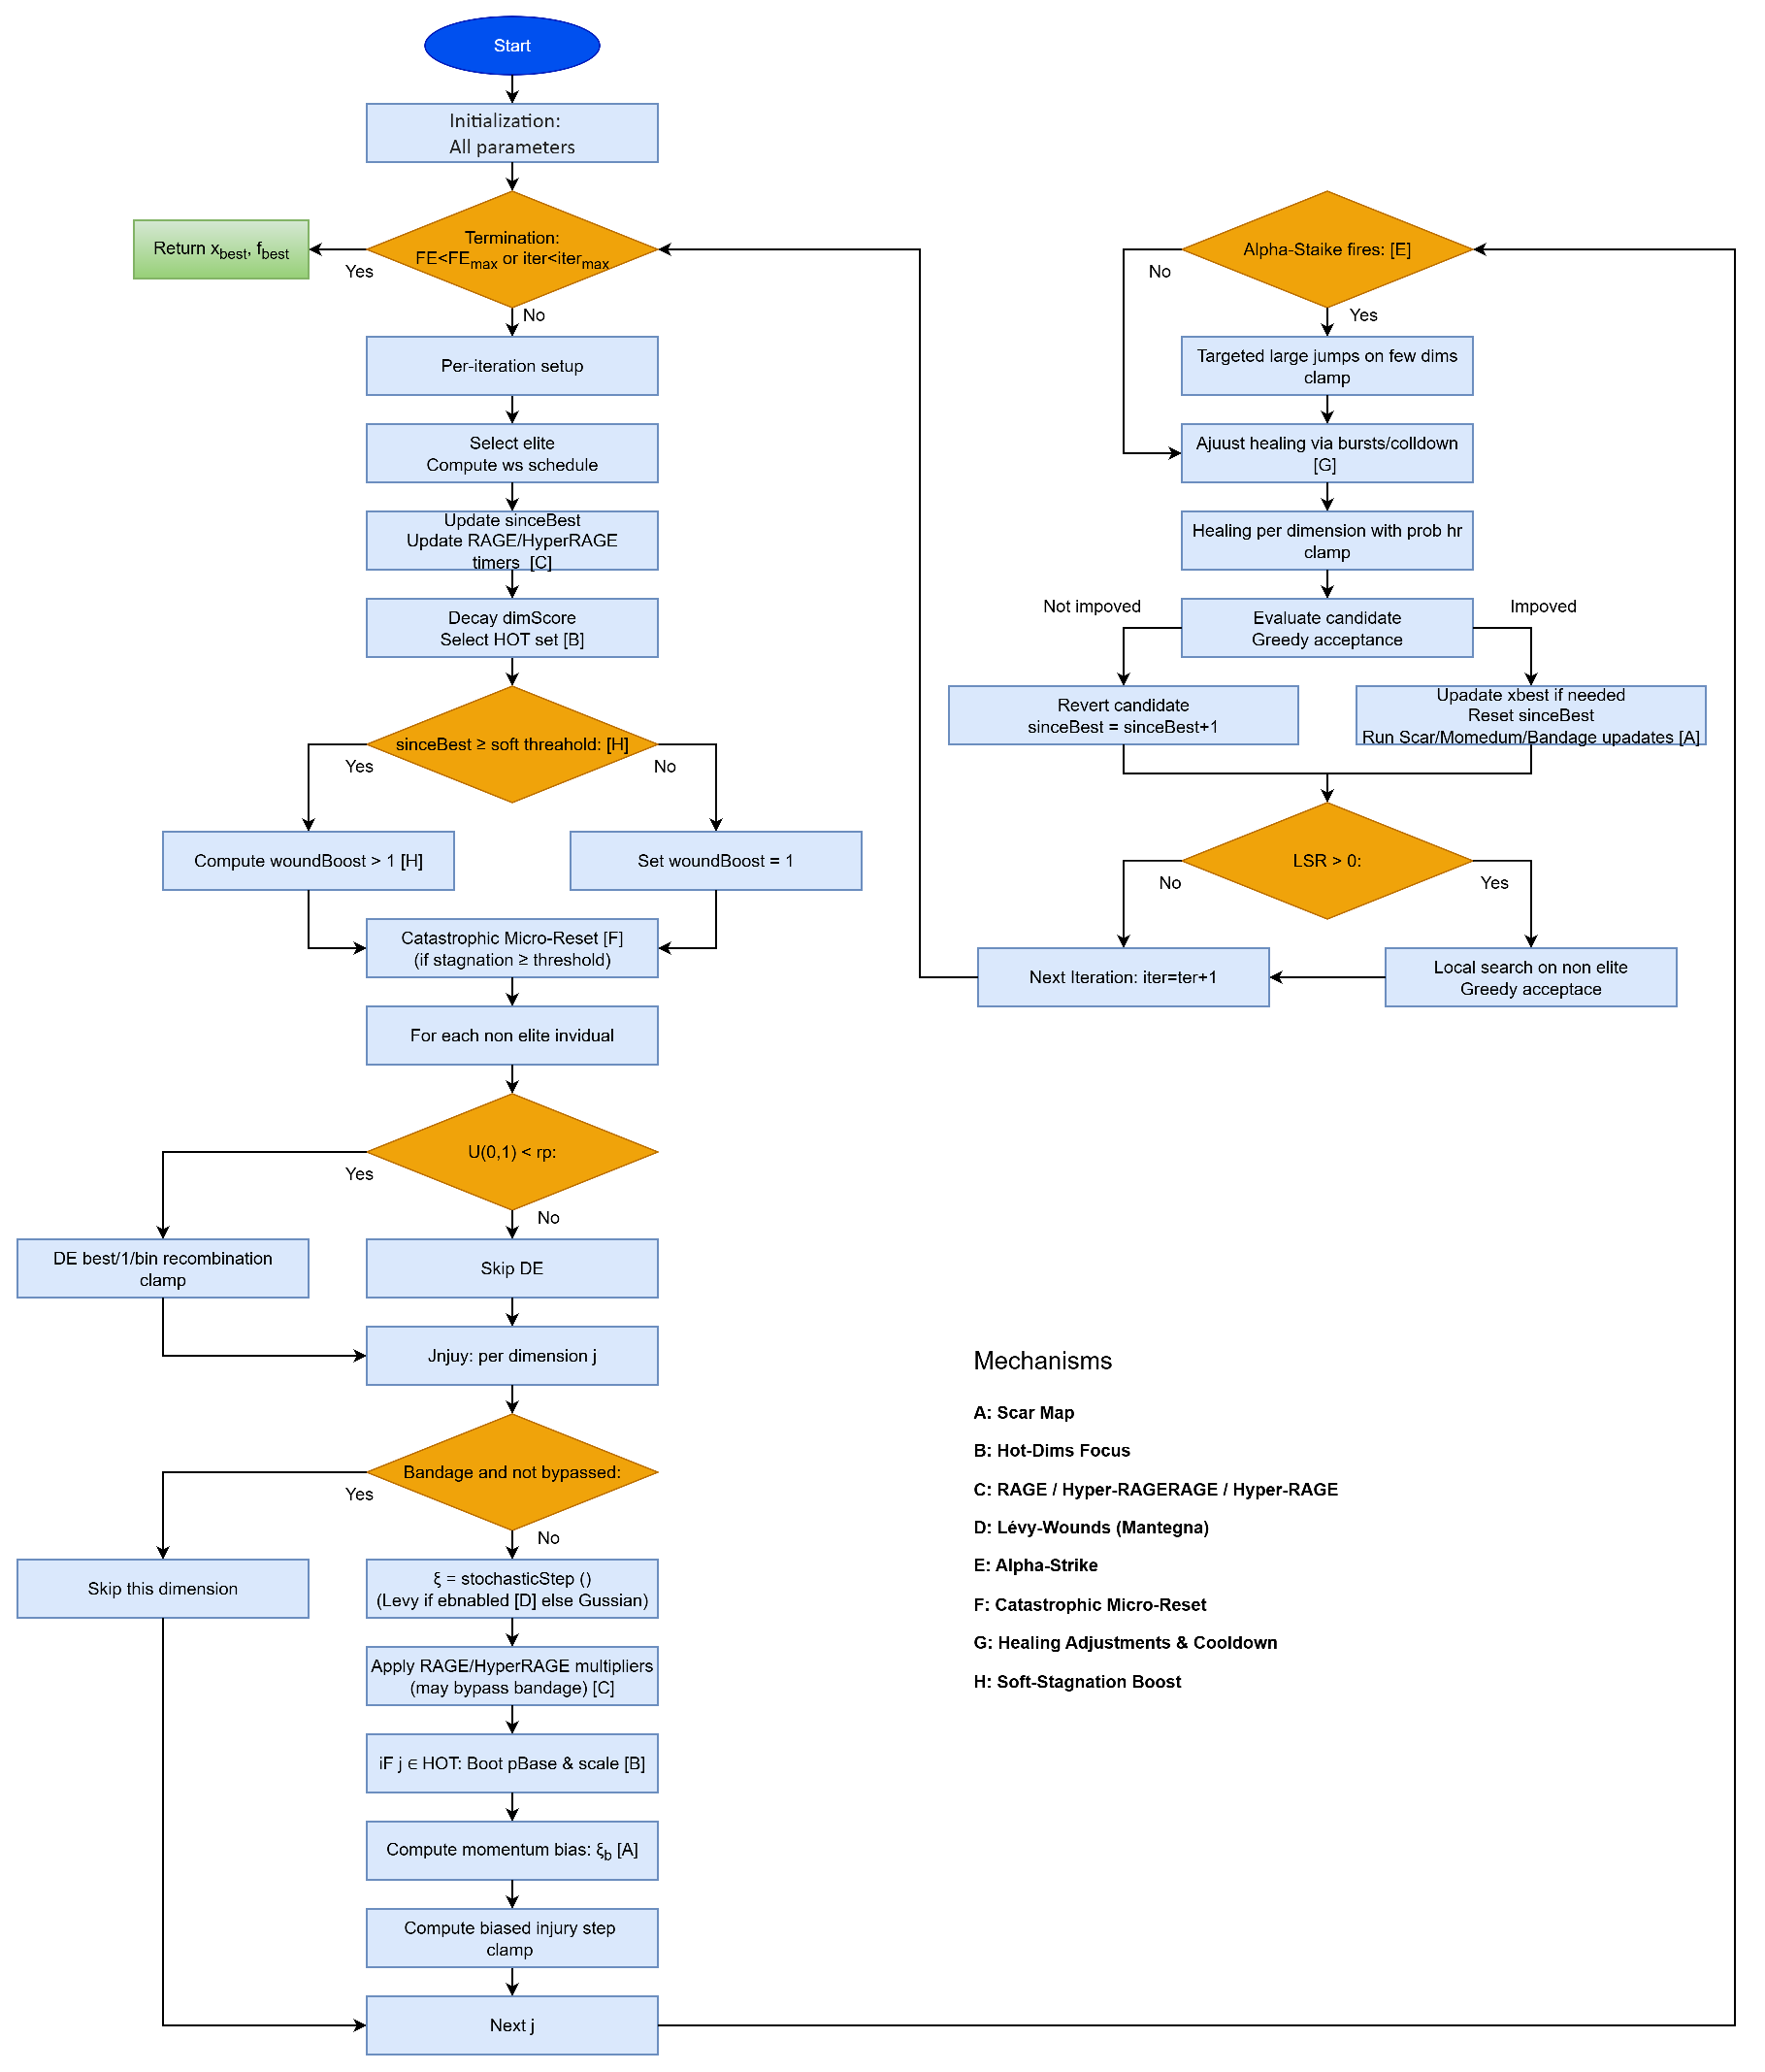
\includegraphics[scale=0.5]{BHO.eps}
\par\end{centering}
\caption{BHO Flowchart: Core Algorithm and Mechanism Integration\label{fig: flowchart}}
\end{figure}


\section{Experimental setup and benchmark results \label{sec:Results}}

This section first introduces the benchmark functions selected for
experimental evaluation, followed by a comprehensive analysis of the
conducted experiments. The study systematically examines the various
parameters of the proposed algorithm to assess its reliability and
effectiveness in different optimization scenarios. The complete parameter
configurations used throughout these experiments are documented in
Table \ref{tab:settings}.

\begin{table}[H]
\caption{Parameters and settings of BHO \label{tab:settings}}

\centering{}{\footnotesize{}%
\begin{tabular}{|c|c|c|}
\hline 
{\footnotesize\textbf{Name}} & {\footnotesize\textbf{Value}} & {\footnotesize\textbf{Description}}\tabularnewline
\hline 
\hline 
{\footnotesize$NP$} & {\footnotesize 100} & {\footnotesize Population size.}\tabularnewline
\hline 
{\footnotesize$iter_{max}$} & {\footnotesize 500} & {\footnotesize Max iterations (also used in ws schedule).}\tabularnewline
\hline 
{\footnotesize$FE_{max}$} & {\footnotesize 150,000} & {\footnotesize Max function evaluations (stopping).}\tabularnewline
\hline 
{\footnotesize$ws_{0}$} & {\footnotesize 0.14} & {\footnotesize Initial injury intensity, decays with iter.}\tabularnewline
\hline 
{\footnotesize$wp$} & {\footnotesize 0.38} & {\footnotesize Per-dimension wounding probability.}\tabularnewline
\hline 
{\footnotesize$hr$} & {\footnotesize 0.8} & {\footnotesize Per-dimension healing probability.}\tabularnewline
\hline 
{\footnotesize$rp$} & {\footnotesize 0.15} & {\footnotesize Probability of DE(best/1,bin) move.}\tabularnewline
\hline 
{\footnotesize$F$} & {\footnotesize 0.7} & {\footnotesize DE scale factor.}\tabularnewline
\hline 
{\footnotesize$CR$} & {\footnotesize 0.5} & {\footnotesize DE crossover rate.}\tabularnewline
\hline 
\multicolumn{3}{|c|}{{\footnotesize\textbf{Scar Map}}}\tabularnewline
\hline 
{\footnotesize$scarBho$} & {\footnotesize yes} & {\footnotesize Enable Scar-Map.}\tabularnewline
\hline 
{\footnotesize$scarLR$} & {\footnotesize 0.06} & {\footnotesize Scar learning rate.}\tabularnewline
\hline 
{\footnotesize$bandage_{len}$} & {\footnotesize 4} & {\footnotesize Freeze improved dims (iters).}\tabularnewline
\hline 
{\footnotesize$scar_{pmin}$/$scar_{pmax}$} & {\footnotesize 0.05 / 0.98} & {\footnotesize Bounds for per-dim wound prob.}\tabularnewline
\hline 
{\footnotesize$scar_{smin}$/$scar_{smax}$} & {\footnotesize 0.50 / 3.00} & {\footnotesize Bounds for per-dim wound scale.}\tabularnewline
\hline 
{\footnotesize$mom_{decay}$} & {\footnotesize 0.25} & {\footnotesize Momentum forgetting rate.}\tabularnewline
\hline 
{\footnotesize$mom_{bias}$} & {\footnotesize 0.75} & {\footnotesize Bias strength toward momentum.}\tabularnewline
\hline 
\multicolumn{3}{|c|}{{\footnotesize\textbf{Hot-Dims Focus}}}\tabularnewline
\hline 
{\footnotesize$dim_{decay}$} & {\footnotesize 0.05} & {\footnotesize Decay rate of dimScore.}\tabularnewline
\hline 
{\footnotesize$hot_{k}$} & {\footnotesize 6} & {\footnotesize Number of top dimensions.}\tabularnewline
\hline 
{\footnotesize$hotBoost_{p}$} & {\footnotesize 1.5} & {\footnotesize Prob. boost on hot dims.}\tabularnewline
\hline 
{\footnotesize$hotBoost_{s}$} & {\footnotesize 1.6} & {\footnotesize Strength boost on hot dims.}\tabularnewline
\hline 
\multicolumn{3}{|c|}{{\footnotesize\textbf{RAGE / Hyper-RAGE}}}\tabularnewline
\hline 
{\footnotesize$rageBho$} & {\footnotesize yes} & {\footnotesize Enable RAGE bursts.}\tabularnewline
\hline 
{\footnotesize$rageStagnThr$} & {\footnotesize 12} & {\footnotesize No-improve threshold for RAGE.}\tabularnewline
\hline 
{\footnotesize$rageLen$} & {\footnotesize 10} & {\footnotesize RAGE duration (iters).}\tabularnewline
\hline 
{\footnotesize$ragePMmult$ / $rageSMmult$} & {\footnotesize 2.2 / 2.8} & {\footnotesize Multipliers for prob/scale in RAGE.}\tabularnewline
\hline 
{\footnotesize$rageIgnoreBandage$} & {\footnotesize yes} & {\footnotesize Ignore bandage during RAGE.}\tabularnewline
\hline 
{\footnotesize$hyperRage$} & {\footnotesize yes} & {\footnotesize Enable Hyper-RAGE.}\tabularnewline
\hline 
{\footnotesize$rage2StagnThr$} & {\footnotesize 28} & {\footnotesize 2nd stagnation threshold.}\tabularnewline
\hline 
{\footnotesize$rage2Len$} & {\footnotesize 12} & {\footnotesize Hyper-RAGE duration.}\tabularnewline
\hline 
{\footnotesize$rage2PMult/rage2SMult$} & {\footnotesize 3.0 / 3.5} & {\footnotesize Multipliers in Hyper-RAGE.}\tabularnewline
\hline 
\multicolumn{3}{|c|}{{\footnotesize\textbf{Lévy-Wounds (Mantegna)}}}\tabularnewline
\hline 
{\footnotesize$levyBho$} & {\footnotesize yes} & {\footnotesize Enable Lévy steps.}\tabularnewline
\hline 
{\footnotesize$levyAlpha$} & {\footnotesize 1.5} & {\footnotesize Tail heaviness parameter.}\tabularnewline
\hline 
{\footnotesize$levyScale$} & {\footnotesize 0.6} & {\footnotesize Lévy step scale.}\tabularnewline
\hline 
\multicolumn{3}{|c|}{{\footnotesize\textbf{Alpha-Strike}}}\tabularnewline
\hline 
{\footnotesize$alphaStrikeRate$} & {\footnotesize 0.1} & {\footnotesize Chance of Alpha-Strike.}\tabularnewline
\hline 
{\footnotesize$alphaStrikeScale$} & {\footnotesize 0.9} & {\footnotesize Alpha-Strike step scale.}\tabularnewline
\hline 
\multicolumn{3}{|c|}{{\footnotesize\textbf{Catastrophic Micro-Reset}}}\tabularnewline
\hline 
{\footnotesize$catReset$} & {\footnotesize yes} & {\footnotesize Enable catastrophic micro-reset.}\tabularnewline
\hline 
{\footnotesize$catResetThr$} & {\footnotesize 40} & {\footnotesize No-improve iters → reset.}\tabularnewline
\hline 
{\footnotesize$catResetFrac$} & {\footnotesize 0.08} & {\footnotesize Fraction of pop to reset.}\tabularnewline
\hline 
{\footnotesize$catSigma$} & {\footnotesize 0.25} & {\footnotesize Sigma around best for reset.}\tabularnewline
\hline 
\multicolumn{3}{|c|}{{\footnotesize\textbf{Healing Adjustments \& Cooldown}}}\tabularnewline
\hline 
{\footnotesize$healRageReduce$} & {\footnotesize 0.35} & {\footnotesize Reduce healing rate in bursts.}\tabularnewline
\hline 
{\footnotesize$healPostCool$} & {\footnotesize 0.25} & {\footnotesize Increase healing after bursts.}\tabularnewline
\hline 
{\footnotesize$cooldownLen$} & {\footnotesize 8} & {\footnotesize Cooldown iterations after bursts.}\tabularnewline
\hline 
\multicolumn{3}{|c|}{{\footnotesize\textbf{Soft-Stagnation Boost}}}\tabularnewline
\hline 
{\footnotesize$stagnThrSoft$} & {\footnotesize 10} & {\footnotesize Soft stagnation threshold.}\tabularnewline
\hline 
{\footnotesize$stagnBoost$} & {\footnotesize 0.4} & {\footnotesize Extra wound factor when soft-stagnant.}\tabularnewline
\hline 
\end{tabular}}{\footnotesize\par}
\end{table}

\begin{table}[H]
\caption{Parameters and settings of other methods\label{tab:settings2}}

\begin{centering}
\begin{tabular}{|c|c|c|}
\hline 
\textbf{Name} & \textbf{Value} & \textbf{Description}\tabularnewline
\hline 
\hline 
$NP$ & 100 & Population size for all methods\tabularnewline
\hline 
$iter_{max}$ & 500 & Maximum number of iterations for all methods\tabularnewline
\hline 
\multicolumn{3}{|c|}{\textbf{CLPSO}}\tabularnewline
\hline 
clProb & 0.3 & Comprehensive learning probability\tabularnewline
\hline 
cognitiveWeight & 1.49445 & Cognitive weight\tabularnewline
\hline 
inertiaWeight & 0.729 & Inertia weight\tabularnewline
\hline 
mutationRate & 0.01 & Mutation rate\tabularnewline
\hline 
socialWeight & 1.49445 & Social weight\tabularnewline
\hline 
\multicolumn{3}{|c|}{\textbf{CMA-ES}}\tabularnewline
\hline 
$NP_{CMA-ES}$ & $4+\left\lfloor 3\cdot\log(dim)\right\rfloor $ & Population size\tabularnewline
\hline 
\multicolumn{3}{|c|}{\textbf{EA4Eig}}\tabularnewline
\hline 
archiveSize & 100 & Archive size for JADE-style mutation\tabularnewline
\hline 
eig\_interval & 5 & Recompute eigenbasis every k iterations\tabularnewline
\hline 
maxCR & 1 & Upper bound for CR\tabularnewline
\hline 
maxF & 1 & Upper bound for F\tabularnewline
\hline 
minCR & 0 & Lower bound for CR\tabularnewline
\hline 
minF & 0.1 & Lower bound for F\tabularnewline
\hline 
pbest & 0.2 & p-best fraction (current-to-pbest/1)\tabularnewline
\hline 
tauCR & 0.1 & Self-adaptation prob. for CR\tabularnewline
\hline 
tauF & 0.1 & Self-adaptation prob. for F\tabularnewline
\hline 
\multicolumn{3}{|c|}{\textbf{mLSHADE\_RL}}\tabularnewline
\hline 
archiveSize & 500 & Archive size\tabularnewline
\hline 
memorySize & 10 & Success-history memory size (H)\tabularnewline
\hline 
minPopulation & 4 & Minimum population size\tabularnewline
\hline 
pmax & 0.2 & Maximum p-best fraction\tabularnewline
\hline 
pmin & 0.05 & Minimum p-best fraction\tabularnewline
\hline 
\multicolumn{3}{|c|}{\textbf{SaDE}}\tabularnewline
\hline 
SaDE.crSigma & 0.1 & Std for CR sampling\tabularnewline
\hline 
SaDE.fGamma & 0.1 & Scale for Cauchy F sampling\tabularnewline
\hline 
SaDE.initCR & 0.5 & Initial CR mean\tabularnewline
\hline 
SaDE.initF & 0.7 & Initial F mean\tabularnewline
\hline 
SaDE.learningPeriod & 25 & Iterations per adaptation window\tabularnewline
\hline 
\multicolumn{3}{|c|}{\textbf{UDE3}}\tabularnewline
\hline 
minPopulation & 4 & Minimum population size. \tabularnewline
\hline 
memorySize & 10 & Success-history memory size (H). \tabularnewline
\hline 
archiveSize & 100 & Archive size. \tabularnewline
\hline 
pmin & 0.05 & Minimum p-best fraction. \tabularnewline
\hline 
pmax & 0.2 & Maximum p-best fraction.\tabularnewline
\hline 
\end{tabular}
\par\end{centering}
\end{table}


\subsection{\textbf{Test Functions \label{subsec:benchmarkFunctions}}}

The performance assessment of the proposed method was carried out
using a comprehensive and diverse collection of well-established benchmark
functions \citep{Siarry,Koyuncu,LaTorre}, as listed in Table \ref{tab:benchmarkFunctions}.
These test functions represent a standard suite commonly utilized
in the global optimization literature for validating and comparing
metaheuristic algorithms. Each function exhibits distinct characteristics
in terms of modality, separability, dimensionality, and landscape
complexity, thus providing a robust basis for evaluating the generalization
capability of the algorithm. Notably, the functions were employed
in their original, unaltered form no additional transformations such
as shifting, rotation, or scaling were applied allowing for a transparent
and reproducible comparison with prior studies.

\begin{table}[H]
\caption{The benchmark functions used in the conducted experiments \label{tab:benchmarkFunctions}}

\centering{}{\tiny{}%
\begin{tabular}{|c|c|c|c|}
\hline 
{\tiny\textbf{PROBLEM}} & {\tiny\textbf{FORMULA}} & {\tiny\textbf{Dim}} & {\tiny\textbf{BOUNDS}}\tabularnewline
\hline 
\hline 
\begin{cellvarwidth}[t]
\centering
{\tiny\textbf{Parameter}}{\tiny\par}

{\tiny\textbf{Estimation for}}{\tiny\par}

{\tiny\textbf{Frequency-Modulated}}{\tiny\par}

{\tiny\textbf{Sound Waves}}
\end{cellvarwidth} & \begin{cellvarwidth}[t]
\centering
{\tiny$\min_{x\in[-6.4,6.35]^{6}}\;f(x)=\frac{1}{N}\sum_{n=1}^{N}\left|y(n;x)-y_{\text{target}}(n)\right|^{2}$}{\tiny\par}

{\tiny$y(n;x)=x_{0}\sin\left(x_{1}n+x_{2}\sin(x_{3}n+x_{4}\sin(x_{5}n))\right)$}
\end{cellvarwidth} & {\tiny 6} & {\tiny$x_{i}\in[-6.4,6.35]$}\tabularnewline
\hline 
\begin{cellvarwidth}[t]
\centering
{\tiny\textbf{Lennard-Jones}}{\tiny\par}

{\tiny\textbf{Potential}}
\end{cellvarwidth} & {\tiny$\min_{x\in\mathbb{R}^{3N-6}}\;f(x)=4\sum_{i=1}^{N-1}\sum_{j=i+1}^{N}\left[\left(\frac{1}{r_{ij}}\right)^{12}-\left(\frac{1}{r_{ij}}\right)^{6}\right]$} & {\tiny 30} & \begin{cellvarwidth}[t]
\centering
{\tiny$x_{0}\in(0,0,0)$}{\tiny\par}

{\tiny$x_{1},x_{2}\in[0,4]$}{\tiny\par}

{\tiny$x_{3}\in[0,\pi]$}{\tiny\par}

{\tiny$x_{3k-3}$}{\tiny\par}

{\tiny$x_{3k-2}$}{\tiny\par}

{\tiny$x_{i}\in[-b_{k},+b_{k}]$}
\end{cellvarwidth}\tabularnewline
\hline 
\begin{cellvarwidth}[t]
\centering
{\tiny\textbf{Bifunctional}}{\tiny\par}

{\tiny\textbf{Catalyst}}{\tiny\par}

{\tiny\textbf{Blend}}{\tiny\par}

{\tiny\textbf{Optimal}}{\tiny\par}

{\tiny\textbf{Control}}
\end{cellvarwidth} & \begin{cellvarwidth}[t]
\centering
{\tiny$\frac{dx_{1}}{dt}=-k_{1}x_{1}$, $\frac{dx_{2}}{dt}=k_{1}x_{1}-k_{2}x_{2}+k_{3}x_{2}+k_{4}x_{3}$,}{\tiny\par}

{\tiny$\frac{dx_{3}}{dt}=k_{2}x_{2}$, $\frac{dx_{4}}{dt}=-k_{4}x_{4}+k_{5}x_{5}$,}{\tiny\par}

{\tiny$\frac{dx_{5}}{dt}=-k_{3}x_{2}+k_{6}x_{4}-k_{5}x_{5}+k_{7}x_{6}+k_{8}x_{7}+k_{9}x_{5}+k_{10}x_{7}$}{\tiny\par}

{\tiny$\frac{dx_{6}}{dt}=k_{8}x_{5}-k_{7}x_{6}$, $\frac{dx_{7}}{dt}=k_{9}x_{5}-k_{10}x_{7}$}{\tiny\par}

{\tiny$k_{i}(u)=c_{i1}+c_{i2}u+c_{i3}u^{2}+c_{i4}u^{3}$}
\end{cellvarwidth} & {\tiny 1} & {\tiny$u\in[0.6,0.9]$}\tabularnewline
\hline 
\begin{cellvarwidth}[t]
\centering
{\tiny\textbf{Optimal}}{\tiny\par}

{\tiny\textbf{Control of a}}{\tiny\par}

{\tiny\textbf{Non-Linear}}{\tiny\par}

{\tiny\textbf{Stirred}}{\tiny\par}

{\tiny\textbf{Tank Reactor}}
\end{cellvarwidth} & \begin{cellvarwidth}[t]
\centering
{\tiny$J(u)=\int_{0}^{0.72}\left[x_{1}(t)^{2}+x_{2}(t)^{2}+0.1u^{2}\right]dt$}{\tiny\par}

{\tiny$\frac{dx_{1}}{dt}=-2x_{1}+x_{2}+1.25u+0.5\exp\left(\frac{x_{1}}{x_{1}+2}\right)$}{\tiny\par}

{\tiny$\frac{dx_{2}}{dt}=-x_{2}+0.5\exp\left(\frac{x_{1}}{x_{1}+2}\right)$}{\tiny\par}

{\tiny$x_{1}(0)=0.9,\quad x_{2}(0)=0.09$, $t\in[0,0.72]$}
\end{cellvarwidth} & {\tiny 1} & {\tiny$u\in[0,5]$}\tabularnewline
\hline 
\begin{cellvarwidth}[t]
\centering
{\tiny\textbf{Tersoff}}{\tiny\par}

{\tiny\textbf{Potential}}{\tiny\par}

{\tiny\textbf{for model Si (B)}}
\end{cellvarwidth} & \begin{cellvarwidth}[t]
\centering
{\tiny$\min_{\mathbf{x}\in\Omega}f(\mathbf{x})=\sum_{i=1}^{N}E(\mathbf{x}_{i})$}{\tiny\par}

{\tiny$E(\mathbf{x}_{i})=\frac{1}{2}\sum_{j\neq i}f_{c}(r_{ij})\left[V_{R}(r_{ij})-B_{ij}V_{A}(r_{ij})\right]$}{\tiny\par}

{\tiny where $r_{ij}=\|\mathbf{x}_{i}-\mathbf{x}_{j}\|$, $V_{R}(r)=A\exp(-\lambda_{1}r)$}{\tiny\par}

{\tiny$V_{A}(r)=B\exp(-\lambda_{2}r)$}{\tiny\par}

{\tiny$f_{c}(r)$: cutoff function with $f_{c}(r)$: angle parameter}
\end{cellvarwidth} & {\tiny 30} & \begin{cellvarwidth}[t]
\centering
{\tiny$x_{1}\in[0,4]$}{\tiny\par}

{\tiny$x_{2}\in[0,4]$}{\tiny\par}

{\tiny$x_{3}\in[0,\pi]$}{\tiny\par}

{\tiny$x_{i}\in\left[\frac{4(i-3)}{4},\ 4\right]$}
\end{cellvarwidth}\tabularnewline
\hline 
\begin{cellvarwidth}[t]
\centering
{\tiny\textbf{Tersoff}}{\tiny\par}

{\tiny\textbf{Potential}}{\tiny\par}

{\tiny\textbf{for model Si (C)}}
\end{cellvarwidth} & \begin{cellvarwidth}[t]
\centering
{\tiny$\min_{\mathbf{x}}\;V(\mathbf{x})=\sum_{i=1}^{N}\sum_{j>i}^{N}f_{C}(r_{ij})\left[a_{ij}f_{R}(r_{ij})+b_{ij}f_{A}(r_{ij})\right]$}{\tiny\par}

{\tiny$f_{C}(r)=\begin{cases}
1, & r<R-D\\
\frac{1}{2}+\frac{1}{2}\cos\left(\frac{\pi(r-R+D)}{2D}\right), & |r-R|\leq D\\
0, & r>R+D
\end{cases}$}{\tiny\par}

{\tiny$f_{R}(r)=A\exp(-\lambda_{1}r)$}{\tiny\par}

{\tiny$f_{A}(r)=-B\exp(-\lambda_{2}r)$}{\tiny\par}

{\tiny$b_{ij}=\left[1+(\beta^{n})\zeta_{ij}^{n}\right]^{-1/(2n)}$}{\tiny\par}

{\tiny$\sum_{k\neq i,j}f_{C}(r_{ik})g(\theta_{ijk})\exp\left[\lambda_{3}^{3}(r_{ij}-r_{ik})^{3}\right]$}
\end{cellvarwidth} & {\tiny 30} & \begin{cellvarwidth}[t]
\centering
{\tiny$x_{1}\in[0,4]$}{\tiny\par}

{\tiny$x_{2}\in[0,4]$}{\tiny\par}

{\tiny$x_{3}\in[0,\pi]$}{\tiny\par}

{\tiny$x_{i}\in\left[\frac{4(i-3)}{4},\ 4\right]$}
\end{cellvarwidth}\tabularnewline
\hline 
\begin{cellvarwidth}[t]
\centering
{\tiny\textbf{Spread}}{\tiny\par}

{\tiny\textbf{Spectrum Radar}}{\tiny\par}

{\tiny\textbf{Polly phase}}{\tiny\par}

{\tiny\textbf{Code Design}}
\end{cellvarwidth} & \begin{cellvarwidth}[t]
\centering
{\tiny$\min_{x\in X}\;f(x)=\max\left\{ |\varphi_{1}(x)|,|\varphi_{2}(x)|,\ldots,|\varphi_{m}(x)|\right\} $}{\tiny\par}

{\tiny$X=\{x\in\mathbb{R}^{n}\mid0\leq x_{j}\leq2\pi,\;j=1,\ldots,n\}m=2n-1$}{\tiny\par}

{\tiny$\varphi_{j}(x)=\begin{cases}
{\displaystyle \sum_{k=1}^{n-j}\cos(x_{k}-x_{k+j})} & \text{for }j=1,\ldots,n-1\\
{\displaystyle n} & \text{for }j=n\\
{\displaystyle \varphi_{2n-j}(x)} & \text{for }j=n+1,\ldots,2n-1
\end{cases}$}{\tiny\par}

{\tiny$\varphi_{j}(x)=\sum_{k=1}^{n-j}\cos(x_{k}-x_{k+j}),\quad j=1,\ldots,n-1$}{\tiny\par}

{\tiny$\varphi_{n}(x)=n$, $\varphi_{n+\ell}(x)=\varphi_{n-\ell}(x),\quad\ell=1,\ldots,n-1$}
\end{cellvarwidth} & {\tiny 20} & {\tiny$x_{j}\in[0,2\pi]$}\tabularnewline
\hline 
\begin{cellvarwidth}[t]
\centering
{\tiny\textbf{Transmission}}{\tiny\par}

{\tiny\textbf{Network}}{\tiny\par}

{\tiny\textbf{Expansion}}{\tiny\par}

{\tiny\textbf{Planning}}
\end{cellvarwidth} & \begin{cellvarwidth}[t]
\centering
{\tiny$\min\sum_{l\in\Omega}c_{l}n_{l}+W_{1}\sum_{l\in OL}|f_{l}-\bar{f}_{l}|+W_{2}\sum_{l\in\Omega}\max(0,n_{l}-\bar{n}_{l})$}{\tiny\par}

{\tiny$Sf=g-d$}{\tiny\par}

{\tiny$f_{l}=\gamma_{l}n_{l}\Delta\theta_{l},\quad\forall l\in\Omega$}{\tiny\par}

{\tiny$|f_{l}|\leq\bar{f}_{l}n_{l},\quad\forall l\in\Omega$}{\tiny\par}

{\tiny$0\leq n_{l}\leq\bar{n}_{l},\quad n_{l}\in\mathbb{Z},\quad\forall l\in\Omega$}
\end{cellvarwidth} & {\tiny 7} & \begin{cellvarwidth}[t]
\centering
{\tiny$0\leq n_{i}\leq\bar{n}_{l}$}{\tiny\par}

{\tiny$n_{i}\in\mathbb{Z}$}
\end{cellvarwidth}\tabularnewline
\hline 
\begin{cellvarwidth}[t]
\centering
{\tiny\textbf{Electricity}}{\tiny\par}

{\tiny\textbf{Transmission}}{\tiny\par}

{\tiny\textbf{Pricing}}
\end{cellvarwidth} & \begin{cellvarwidth}[t]
\centering
{\tiny$\min_{x}\;\;f(x)=\sum_{i=1}^{N_{g}}\left(\frac{C_{i}^{gen}}{P_{i}^{gen}}-R_{i}^{gen}\right)^{2}+\sum_{j=1}^{N_{d}}\left(\frac{C_{j}^{load}}{P_{j}^{load}}-R_{j}^{load}\right)^{2}$}{\tiny\par}

{\tiny$\sum_{j}GD_{i,j}+\sum_{j}BT_{i,j}=P_{i}^{gen},\quad\forall i$}{\tiny\par}

{\tiny$\sum_{i}GD_{i,j}+\sum_{i}BT_{i,j}=P_{j}^{load},\quad\forall j$}{\tiny\par}

{\tiny$GD_{i,j}^{max}=\min(P_{i}^{gen}-BT_{i,j},\;P_{j}^{load}-BT_{i,j})$}
\end{cellvarwidth} & {\tiny 126} & {\tiny$GD_{i,j}\in[0,GD_{i,j}^{max}]$}\tabularnewline
\hline 
\begin{cellvarwidth}[t]
\centering
{\tiny\textbf{Circular}}{\tiny\par}

{\tiny\textbf{Antenna}}{\tiny\par}

{\tiny\textbf{Array}}{\tiny\par}

{\tiny\textbf{Design}}
\end{cellvarwidth} & \begin{cellvarwidth}[t]
\centering
{\tiny$\min_{r_{1},\ldots,r_{6},\,\varphi_{1},\ldots,\varphi_{6}}\quad f(\mathbf{x})=\max_{\theta\in\Omega}AF(\mathbf{x},\theta)$}{\tiny\par}

{\tiny$AF(\mathbf{x},\theta)=\left|\sum_{k=1}^{6}\exp\left(j\left[2\pi r_{k}\cos(\theta-\theta_{k})+\varphi_{k}\frac{\pi}{180}\right]\right)\right|$}
\end{cellvarwidth} & {\tiny 12} & \begin{cellvarwidth}[t]
\centering
{\tiny$r_{k}\in[0.2,1]$}{\tiny\par}

{\tiny$\varphi_{k}\in[-180,180]$}
\end{cellvarwidth}\tabularnewline
\hline 
\begin{cellvarwidth}[t]
\centering
{\tiny\textbf{Dynamic}}{\tiny\par}

{\tiny\textbf{Economic}}{\tiny\par}

{\tiny\textbf{Dispatch 1}}
\end{cellvarwidth} & \begin{cellvarwidth}[t]
\centering
{\tiny$\min_{\mathbf{P}}\quad f(\mathbf{P})=\sum_{t=1}^{24}\sum_{i=1}^{5}\left(a_{i}P_{i,t}^{2}+b_{i}P_{i,t}+c_{i}\right)$}{\tiny\par}

{\tiny$P_{i}^{\min}\leq P_{i,t}\leq P_{i}^{\max},\quad\forall i=1,\ldots,5,\;t=1,\ldots,24$}{\tiny\par}

{\tiny$\sum_{i=1}^{5}P_{i,t}=D_{t},\quad\forall t=1,\ldots,24$}{\tiny\par}

{\tiny$P_{\min}=[10,20,30,40,50]$}{\tiny\par}

{\tiny$P_{\max}=[75,125,175,250,300]$}
\end{cellvarwidth} & {\tiny 120} & {\tiny$P_{i}^{\min}\leq P_{i,t}\leq P_{i}^{\max}$}\tabularnewline
\hline 
\begin{cellvarwidth}[t]
\centering
{\tiny\textbf{Dynamic}}{\tiny\par}

{\tiny\textbf{Economic}}{\tiny\par}

{\tiny\textbf{Dispatch 2}}
\end{cellvarwidth} & \begin{cellvarwidth}[t]
\centering
{\tiny$\min_{\mathbf{P}}\quad f(\mathbf{P})=\sum_{t=1}^{24}\sum_{i=1}^{9}\left(a_{i}P_{i,t}^{2}+b_{i}P_{i,t}+c_{i}\right)$}{\tiny\par}

{\tiny$P_{i}^{\min}\leq P_{i,t}\leq P_{i}^{\max},\quad\forall i=1,\ldots,5,\;t=1,\ldots,24$}{\tiny\par}

{\tiny$\sum_{i=1}^{5}P_{i,t}=D_{t},\quad\forall t=1,\ldots,24$}{\tiny\par}

{\tiny$P_{\min}=[150,135,73,60,73,57,20,47,20]$}{\tiny\par}

{\tiny$P_{\max}=[470,460,340,300,243,160,130,120,80]$}
\end{cellvarwidth} & {\tiny 216} & {\tiny$P_{i}^{\min}\leq P_{i,t}\leq P_{i}^{\max}$}\tabularnewline
\hline 
\begin{cellvarwidth}[t]
\centering
{\tiny\textbf{Static}}{\tiny\par}

{\tiny\textbf{Economic}}{\tiny\par}

{\tiny\textbf{Load}}{\tiny\par}

{\tiny\textbf{Dispatch}}{\tiny\par}

{\tiny\textbf{(1,2,3,4,5)}}
\end{cellvarwidth} & \begin{cellvarwidth}[t]
\centering
{\tiny$\min_{P_{1},\ldots,P_{N_{G}}}F=\sum_{i=1}^{N_{G}}f_{i}(P_{i})$}{\tiny\par}

{\tiny$f_{i}(P_{i})=a_{i}P_{i}^{2}+b_{i}P_{i}+c_{i},\quad i=1,2,\ldots,N_{G}$}{\tiny\par}

{\tiny$f_{i}(P_{i})=a_{i}P_{i}^{2}+b_{i}P_{i}+c_{i}+|e_{i}\sin(f_{i}(P_{i}^{\min}-P_{i}))|$}{\tiny\par}

{\tiny$P_{i}^{\min}\leq P_{i}\leq P_{i}^{\max},\quad i=1,2,\ldots,N_{G}$}{\tiny\par}

{\tiny$\sum_{i=1}^{N_{G}}P_{i}=P_{D}+P_{L}$}{\tiny\par}

{\tiny$P_{L}=\sum_{i=1}^{N_{G}}\sum_{j=1}^{N_{G}}P_{i}B_{ij}P_{j}+\sum_{i=1}^{N_{G}}B_{0i}P_{i}+B_{00}$}{\tiny\par}

{\tiny$P_{i}-P_{i}^{0}\leq UR_{i}\quad P_{i}^{0}-P_{i}\leq DR_{i}$}
\end{cellvarwidth} & \begin{cellvarwidth}[t]
\centering
{\tiny 6}{\tiny\par}

{\tiny 13}{\tiny\par}

{\tiny 15}{\tiny\par}

{\tiny 40}{\tiny\par}

{\tiny 140}
\end{cellvarwidth} & \begin{cellvarwidth}[t]
\centering
{\tiny See}{\tiny\par}

{\tiny Technical}{\tiny\par}

{\tiny Report}{\tiny\par}

{\tiny of}{\tiny\par}

{\tiny CEC2011}
\end{cellvarwidth}\tabularnewline
\hline 
\end{tabular}}{\tiny\par}
\end{table}


\subsection{\textbf{Experimental results\label{subsec:experimentalResults}} }

All experimental procedures were executed on a high-performance computational
infrastructure equipped with an AMD Ryzen 9 5950X CPU (16 cores, 32
threads) and 128 GB of DDR4 RAM, running under a Debian Linux environment.
The evaluation protocol was designed to ensure statistical rigor and
reproducibility. Specifically, each benchmark function was subjected
to 30 independent runs, with each trial initialized using distinct
random seeds to account for stochastic variability in the algorithm’s
behavior.

The BioHealingOptimizer and all comparative methods were implemented
in highly optimized ANSI C++ code, integrated into the GLOBALOPTIMUS
optimization framework \citep{Tsoulos}, which is an open-source software
environment for metaheuristic experimentation. The source code is
publicly available at https://github.com/itsoulos/GLOBALOPTIMUS (accessed
August 1, 2025), promoting transparency and reproducibility in research.

All algorithmic parameters, including those of competing methods,
are comprehensively outlined in Tables \ref{tab:settings} and \ref{tab:settings2}.
The primary performance metric reported is the average number of objective
function evaluations (NFEs) computed over the 30 runs for each test
function. Additionally, success rates defined as the percentage of
runs in which the global optimum was successfully located are included
in parentheses next to the corresponding mean values. In cases where
all runs achieved optimal convergence, the success rate indicator
is omitted for clarity. Within the result tables, best-performing
entries (i.e., those requiring the fewest function evaluations) are
visually highlighted in green to facilitate comparison.

For the experimental evaluation of BHO, we selected the following
optimization algorithms as baselines for comparison:
\begin{itemize}
\item EA4Eig \citep{key-1} is a cooperative evolutionary algorithm with
an eigen--crossover operator, introduced at IEEE CEC 2022 and evaluated
on that event’s benchmark suite it was essentially designed and tested
within the CEC single-objective context.
\item UDE3 (UDE-III) \citep{key-2} is a recent member of the Unified DE
family for constrained problems it is evaluated on the CEC 2024 constrained
set, while its predecessor (UDE-II/IUDE) won first place at CEC 2018,
giving UDE3 a clear lineage with proven competitive performance.
\item mLSHADE\_RL \citep{key-3} is a multi-operator descendant of LSHADE-cnEpSin
one of the CEC 2017 winners for real-parameter optimizationaugmenting
the base with restarts and local search and being assessed on modern
test suites.
\item CLPSO \citep{key-4} is a classic PSO variant with comprehensive learning
(2006) that has long served as a strong baseline in CEC benchmarks,
not tied to a single award entry but widely used in comparative studies.
\item SaDE, \citep{key-5} the self-adaptive DE of Qin \& Suganthan, was
presented with evaluation on the CEC 2005 test set and has since become
a reference point for adaptive strategies.
\item jDE \citep{key-6} by Brest et al. introduced self-adaptation of F
and CR and was extensively evaluated, including special CEC 2009 sessions
on dynamic/uncertain optimization, helping popularize self-adaptation
in DE.
\item CMA-ES \citep{key-7} is the established covariance matrix adaptation
evolution strategy for continuous domains beyond its vast literature,
it is a staple baseline and frequent participant/reference in BBOB
benchmarking at GECCO, effectively serving as a de facto competitive
black-box comparison standard.
\end{itemize}
\begin{sidewaystable}[H]
\caption{Algorithms’ Comparison Based on Best and Mean after 1.5e+5 FEs \label{tab:algorithms}}

\centering{}{\tiny{}%
\begin{tabular}{|c|c|c|c|c|c|c|c|c|c|c|c|c|c|c|c|c|}
\hline 
{\tiny FUNCTION} & {\tiny EA4Eig best} & {\tiny EA4Eig mean} & {\tiny UDE3 best} & {\tiny UDE3 mean} & {\tiny mLSHADE\_RL best} & {\tiny mLSHADE\_RL mean} & {\tiny CLPSO best} & {\tiny CLPSO mean} & {\tiny SaDE best} & {\tiny SaDE mean} & {\tiny jDE best} & {\tiny jDE mean} & {\tiny CMA-ES best} & {\tiny CMA-ES mean} & {\tiny BHO best} & {\tiny BHO mean}\tabularnewline
\hline 
\hline 
\begin{cellvarwidth}[t]
\centering
{\tiny\textbf{Parameter}}{\tiny\par}

{\tiny\textbf{Estimation for}}{\tiny\par}

{\tiny\textbf{Frequency-Modulated}}{\tiny\par}

{\tiny\textbf{Sound Waves}}
\end{cellvarwidth} & {\tiny 0.153993305} & {\tiny 0.213447296} & {\tiny 0.03808755} & {\tiny 0.115833815} & {\tiny 0.116157535} & {\tiny 0.205011062} & {\tiny 0.1314837477} & {\tiny 0.2124981688} & {\tiny 0.095829444} & {\tiny 0.195600253} & {\tiny 0.116157541} & {\tiny 0.146008756} & {\tiny 0.18160916} & {\tiny 0.256863966} & {\tiny 1.543773917e-25} & {\tiny 0.200220764}\tabularnewline
\hline 
\begin{cellvarwidth}[t]
\centering
{\tiny\textbf{Lennard-Jones}}{\tiny\par}

{\tiny\textbf{Potential}}
\end{cellvarwidth} & {\tiny -18.48174236} & {\tiny -16.3133561} & {\tiny -21.41786661} & {\tiny -17.33977959} & {\tiny -28.41816707} & {\tiny -22.49792055} & {\tiny -13.43649135} & {\tiny -10.25073403} & {\tiny -21.93636189} & {\tiny -17.95333019} & {\tiny -29.98126575} & {\tiny -27.49258505} & {\tiny -28.42253189} & {\tiny -25.78783328} & {\tiny -32.07742417} & {\tiny -24.33212306}\tabularnewline
\hline 
\begin{cellvarwidth}[t]
\centering
{\tiny\textbf{Bifunctional}}{\tiny\par}

{\tiny\textbf{Catalyst Blend}}{\tiny\par}

{\tiny\textbf{Optimal Control}}
\end{cellvarwidth} & {\tiny -0.000286591} & {\tiny -0.000286591} & {\tiny -0.000286591} & {\tiny -0.000286591} & {\tiny -0.000286591} & {\tiny -0.000286591} & {\tiny -0.000286591} & {\tiny -0.000286591} & {\tiny -0.000286591} & {\tiny -0.000286591} & {\tiny -0.000286591} & {\tiny -0.000286591} & {\tiny -0.000286591} & {\tiny -0.000286591} & {\tiny -0.000286591} & {\tiny -0.000286591}\tabularnewline
\hline 
\begin{cellvarwidth}[t]
\centering
{\tiny\textbf{Optimal Control of a}}{\tiny\par}

{\tiny\textbf{Non-Linear Stirred}}{\tiny\par}

{\tiny\textbf{Tank Reactor}}
\end{cellvarwidth} & {\tiny 0.390376723} & {\tiny 0.390376723} & {\tiny 0.390376723} & {\tiny 0.390376723} & {\tiny 0.390376723} & {\tiny 0.390376723} & {\tiny 0.3903767228} & {\tiny 0.3903767228} & {\tiny 0.390376723} & {\tiny 0.390376723} & {\tiny 0.390376723} & {\tiny 0.390376723} & {\tiny 0.3903767228} & {\tiny 0.390376723} & {\tiny 0.3903767228} & {\tiny 0.390376723}\tabularnewline
\hline 
\begin{cellvarwidth}[t]
\centering
{\tiny\textbf{Tersoff Potential}}{\tiny\par}

{\tiny\textbf{for model Si (B)}}
\end{cellvarwidth} & {\tiny -29.11960284} & {\tiny -27.89597789} & {\tiny -29.44152761} & {\tiny -25.70627602} & {\tiny -28.60814558} & {\tiny -26.07976794} & {\tiny -28.23544117} & {\tiny -26.18834522} & {\tiny -27.25703406} & {\tiny -25.25867422} & {\tiny -13.51157064} & {\tiny -3.983690794} & {\tiny -29.26244222} & {\tiny -27.5889735} & {\tiny -29.03183049} & {\tiny -27.26630121}\tabularnewline
\hline 
\begin{cellvarwidth}[t]
\centering
{\tiny\textbf{Tersoff Potential}}{\tiny\par}

{\tiny\textbf{for model Si (C)}}
\end{cellvarwidth} & {\tiny -33.39767521} & {\tiny -31.11610936} & {\tiny -33.12997729} & {\tiny -28.6603137} & {\tiny -32.28575942} & {\tiny -30.03594436} & {\tiny -30.85200257} & {\tiny -28.87349048} & {\tiny -31.85343594} & {\tiny -29.59692733} & {\tiny -18.76214649} & {\tiny -8.506037168} & {\tiny -33.19699356} & {\tiny -31.79270914} & {\tiny -33.38947338} & {\tiny -31.31864105}\tabularnewline
\hline 
\begin{cellvarwidth}[t]
\centering
{\tiny\textbf{Spread Spectrum}}{\tiny\par}

{\tiny\textbf{Radar Polly phase}}{\tiny\par}

{\tiny\textbf{Code Design}}
\end{cellvarwidth} & {\tiny 0.517866993} & {\tiny 0.838752978} & {\tiny 1.048240196} & {\tiny 1.265152951} & {\tiny 0.033146096} & {\tiny 0.625788451} & {\tiny 1.085334991} & {\tiny 1.343956153} & {\tiny 0.572731322} & {\tiny 0.844014075} & {\tiny 1.525870558} & {\tiny 1.812042166} & {\tiny 0.01484822722} & {\tiny 0.171988666} & {\tiny 0.195096433} & {\tiny 0.601190863}\tabularnewline
\hline 
\begin{cellvarwidth}[t]
\centering
{\tiny\textbf{Transmission Network}}{\tiny\par}

{\tiny\textbf{Expansion Planning}}
\end{cellvarwidth} & {\tiny 250} & {\tiny 250} & {\tiny 250} & {\tiny 250} & {\tiny 250} & {\tiny 250} & {\tiny 250} & {\tiny 250} & {\tiny 250} & {\tiny 250} & {\tiny 250} & {\tiny 250} & {\tiny 250} & {\tiny 250} & {\tiny 250} & {\tiny 250}\tabularnewline
\hline 
\begin{cellvarwidth}[t]
\centering
{\tiny\textbf{Electricity}}{\tiny\par}

{\tiny\textbf{Transmission Pricing}}
\end{cellvarwidth} & {\tiny 13773680} & {\tiny 13774198.28} & {\tiny 13773582.53} & {\tiny 13773582.53} & {\tiny 13773567.36} & {\tiny 13773852.63} & {\tiny 13775010.1} & {\tiny 13775395.07} & {\tiny 13773468.68} & {\tiny 13773930.93} & {\tiny 13774627.84} & {\tiny 14020953.78} & {\tiny 13775841.77} & {\tiny 13787550.18} & {\tiny 13773334.9} & {\tiny 13773632.45}\tabularnewline
\hline 
\begin{cellvarwidth}[t]
\centering
{\tiny\textbf{Circular Antenna}}{\tiny\par}

{\tiny\textbf{Array Design}}
\end{cellvarwidth} & {\tiny 0.006809638} & {\tiny 0.006809638} & {\tiny 0.006809653} & {\tiny 0.011722944} & {\tiny 0.006809701} & {\tiny 0.006823547} & {\tiny 0.006933401045} & {\tiny 0.05181551798} & {\tiny 0.00681287} & {\tiny 0.008186204} & {\tiny 0.006820072} & {\tiny 0.017657998} & {\tiny 0.007204797576} & {\tiny 0.008635655364} & {\tiny 0.007101505} & {\tiny 0.158523549}\tabularnewline
\hline 
\begin{cellvarwidth}[t]
\centering
{\tiny\textbf{Dynamic Economic}}{\tiny\par}

{\tiny\textbf{Dispatch 1}}
\end{cellvarwidth} & {\tiny 412736103.9} & {\tiny 421199260.5} & {\tiny 410197836.9} & {\tiny 410628483.3} & {\tiny 415275891.6} & {\tiny 418526775.3} & {\tiny 428607927.6} & {\tiny 435250914.5} & {\tiny 411226317.3} & {\tiny 413699347.4} & {\tiny 968042312.1} & {\tiny 1034393036} & {\tiny 88285.6024} & {\tiny 102776.7103} & {\tiny 410074526.4} & {\tiny 410079513.3}\tabularnewline
\hline 
\begin{cellvarwidth}[t]
\centering
{\tiny\textbf{Dynamic Economic}}{\tiny\par}

{\tiny\textbf{Dispatch 2}}
\end{cellvarwidth} & {\tiny 346855.5418} & {\tiny 12332507.25} & {\tiny 357530.5408} & {\tiny 537163.4139} & {\tiny 392247.7213} & {\tiny 5966956.365} & {\tiny 33031590.31} & {\tiny 53906147.38} & {\tiny 519820.5596} & {\tiny 4090304.18} & {\tiny 340091475.3} & {\tiny 397471715.1} & {\tiny 502699.4187} & {\tiny 477720.1511} & {\tiny 347469.862} & {\tiny 354734.7105}\tabularnewline
\hline 
\begin{cellvarwidth}[t]
\centering
{\tiny\textbf{StaticEconomic}}{\tiny\par}

{\tiny\textbf{Load Dispatch 1}}
\end{cellvarwidth} & {\tiny 6163.560978} & {\tiny 6170.965013} & {\tiny 6164.766919} & {\tiny 6266.250251} & {\tiny 6163.546883} & {\tiny 6353.722019} & {\tiny 6554.672173} & {\tiny 7668.333603} & {\tiny 6360.353305} & {\tiny 6464.861828} & {\tiny 6163.749006} & {\tiny 6778.527028} & {\tiny 6657.613028} & {\tiny 415917.4625} & {\tiny 6512.525519} & {\tiny 6772.880257}\tabularnewline
\hline 
\begin{cellvarwidth}[t]
\centering
{\tiny\textbf{Static Economic}}{\tiny\par}

{\tiny\textbf{Load Dispatch 2}}
\end{cellvarwidth} & {\tiny 14.46160489} & {\tiny 18779.92036} & {\tiny 18725.64707} & {\tiny 19660.49074} & {\tiny 17905.85383} & {\tiny 18661.20763} & {\tiny 19030.36081} & {\tiny 20699.00219} & {\tiny 18455.37286} & {\tiny 21829.10208} & {\tiny 1161578.904} & {\tiny 3671587.605} & {\tiny 763001.2185} & {\tiny 1425815.44} & {\tiny 18754.99866} & {\tiny 19232.05211}\tabularnewline
\hline 
\begin{cellvarwidth}[t]
\centering
{\tiny\textbf{Static Economic}}{\tiny\par}

{\tiny\textbf{Load Dispatch 3}}
\end{cellvarwidth} & {\tiny 470023232.3} & {\tiny 470023234.5} & {\tiny 470023232.3} & {\tiny 470023232.3} & {\tiny 470023232.6} & {\tiny 470023234.7} & {\tiny 470192288.3} & {\tiny 470294703.2} & {\tiny 470023232.7} & {\tiny 470023232.7} & {\tiny 471058115.8} & {\tiny 471963142.3} & {\tiny 470023232.3} & {\tiny 470023232.3} & {\tiny 470023233.2} & {\tiny 470023278}\tabularnewline
\hline 
\begin{cellvarwidth}[t]
\centering
{\tiny\textbf{Static Economic}}{\tiny\par}

{\tiny\textbf{Load Dispatch 4}}
\end{cellvarwidth} & {\tiny 71193.07649} & {\tiny 71193.07649} & {\tiny 168334.7003} & {\tiny 348720.6677} & {\tiny 71067.8441} & {\tiny 406986.2181} & {\tiny 884980.5569} & {\tiny 1423887.358} & {\tiny 862196.432} & {\tiny 1469886.142} & {\tiny 6482592.714} & {\tiny 17527314.24} & {\tiny 476053.5197} & {\tiny 2925852.935} & {\tiny 71089.03508} & {\tiny 100831.805}\tabularnewline
\hline 
\begin{cellvarwidth}[t]
\centering
{\tiny\textbf{Static Economic}}{\tiny\par}

{\tiny\textbf{Load Dispatch 15}}
\end{cellvarwidth} & {\tiny 8085796774} & {\tiny 8145304780} & {\tiny 8070408727} & {\tiny 8071802922} & {\tiny 8079118012} & {\tiny 8104455647} & {\tiny 8105947615} & {\tiny 8110924071} & {\tiny 8078489742} & {\tiny 8081680478} & {\tiny 8453090778} & {\tiny 8459337082} & {\tiny 8072077963} & {\tiny 8084017791} & {\tiny 8072061692} & {\tiny 74458095}\tabularnewline
\hline 
\end{tabular}}{\tiny\par}
\end{sidewaystable}

On synthetic and physical potentials, BHO delivers particularly strong
best values nearly zero error on Parameter Estimation for Frequency-Modulated
Sound Waves and attains the lowest best value on the Lennard-Jones
Potential however, for the mean on Lennard-Jones, jDE leads and CMA-ES
follows, indicating that classical, Gaussian-driven strategies remain
very stable when the landscape exhibits symmetric curvature. On the
Tersoff Potential for model Si (B) and Tersoff Potential for model
Si (C) the picture shifts: for Si (B) the best mean comes from EA4Eig
with CMA-ES close behind, while UDE3 secures the best best for Si
(C), EA4Eig has the best best and CMA-ES the best mean. Overall, advanced
DE variants with stronger recombination (EA4Eig, UDE3) and CMA-ES
alternate at the top, which aligns with the literature on rough but
moderately structured landscapes.

In electro-economic and industrial test cases the pattern diverges
in informative ways. On Electricity Transmission Pricing, BHO attains
the lowest best, whereas UDE3 achieves the best mean suggesting BHO
can hit excellent extremes while UDE3 maintains consistently low performance
across runs. In Dynamic Economic Dispatch 1 and Dynamic Economic Dispatch
2, CMA-ES dominates the first on both best and mean, confirming its
strength on smooth, nearly quadratic geometries, while in the second
BHO records the lowest mean and EA4Eig the best best, indicating that
BHO’s injury--healing dynamics act as a variance-damping safety net.
Across the static dispatch family the results are mixed: in StaticEconomic
Load Dispatch 1 the best best is from mLSHADE\_RL and the best mean
from EA4Eig in Static Economic Load Dispatch 2 mLSHADE\_RL yields
the lowest mean (with EA4Eig taking the best best) in Static Economic
Load Dispatch 4 mLSHADE\_RL again takes the best best while EA4Eig
leads on mean. Static Economic Load Dispatch 3 shows practical ties
around the same value and is not very discriminative. Static Economic
Load Dispatch 15 contains a notable outlier where BHO’s mean is orders
of magnitude lower than others this merits independent verification,
such as re-running experiments or checking units, because the unusually
large gap likely signals a scaling difference or an unexpected effect.

On more “classic” comparative tests, CMA-ES shows impressive robustness
on smooth, well-scaled landscapes: beyond Dynamic Economic Dispatch
1, it also holds both best and mean on Spread Spectrum Radar Polly
phase Code Design. EA4Eig stands out when strong anisotropy or correlation
matters Circular Antenna Array Design is topped by EA4Eig on both
best and mean consistent with its eigen-crossover design. UDE3 performs
very well on problems with additional structure or constraints, such
as the mean on Electricity Transmission Pricing, matching its remit
as a unified DE for constrained scenarios. mLSHADE\_RL frequently
attains best-case wins in StaticEconomic Load Dispatch 1 and Static
Economic Load Dispatch 4 and remains competitive on mean across several
cases, underscoring the value of ensemble mutation plus restarts on
fractured landscapes. SaDE, while a solid baseline, tends to trail
the newer DE descendants, and CLPSO underperforms in most tables expected
where anisotropy demands directional information beyond standard swarm
velocity updates. jDE remains competitive on certain physical potentials,
for example the mean on Lennard-Jones, but shows larger dispersion
on industrial dispatch tasks.

On flat or near-flat landscapes Bifunctional Catalyst Blend Optimal
Control, Transmission Network Expansion Planning, and essentially
Optimal Control of a Non-Linear Stirred Tank Reactor where differences
are on the order of 1e-10 all methods tie or are practically indistinguishable,
so these tests add little diagnostic power. In sum, there is no single
winner: CMA-ES is the reference choice for smooth, well-conditioned
cases and remains very strong on mean performance EA4Eig excels where
alignment with principal variance directions helps UDE3 often wins
on mean under constrained or pricing structure mLSHADE\_RL frequently
takes best-case wins on difficult static dispatch variants and BHO
shows top best values on several critical functions and competitive
means in demanding settings, indicating an effective exploration-to-exploitation
transition.
\begin{table}[H]
\caption{Detailed Ranking of Algorithms Based on Best after 1.5e+5 FEs \label{tab:rankingBest}}

\centering{}{\footnotesize{}%
\begin{tabular}{|c|c|c|c|c|c|c|c|c|}
\hline 
{\footnotesize\textbf{FUNCTION}} & {\footnotesize\textbf{EA4Eig}} & {\footnotesize\textbf{UDE3}} & {\footnotesize\textbf{mLSHADE\_RL}} & {\footnotesize\textbf{CLPSO}} & {\footnotesize\textbf{SaDE}} & {\footnotesize\textbf{jDE}} & {\footnotesize\textbf{CMA-ES}} & {\footnotesize\textbf{BHO}}\tabularnewline
\hline 
\hline 
\begin{cellvarwidth}[t]
\centering
{\tiny\textbf{Parameter}}{\tiny\par}

{\tiny\textbf{Estimation for}}{\tiny\par}

{\tiny\textbf{Frequency-Modulated}}{\tiny\par}

{\tiny\textbf{Sound Waves}}
\end{cellvarwidth} & {\footnotesize 7} & {\footnotesize 2} & {\footnotesize 4} & {\footnotesize 6} & {\footnotesize 3} & {\footnotesize 5} & {\footnotesize 8} & {\footnotesize 1}\tabularnewline
\hline 
\begin{cellvarwidth}[t]
\centering
{\tiny\textbf{Lennard-Jones}}{\tiny\par}

{\tiny\textbf{Potential}}
\end{cellvarwidth} & {\footnotesize 7} & {\footnotesize 6} & {\footnotesize 4} & {\footnotesize 8} & {\footnotesize 5} & {\footnotesize 2} & {\footnotesize 3} & {\footnotesize 1}\tabularnewline
\hline 
\begin{cellvarwidth}[t]
\centering
{\tiny\textbf{Bifunctional}}{\tiny\par}

{\tiny\textbf{Catalyst Blend}}{\tiny\par}

{\tiny\textbf{Optimal Control}}
\end{cellvarwidth} & {\footnotesize 1} & {\footnotesize 1} & {\footnotesize 1} & {\footnotesize 1} & {\footnotesize 1} & {\footnotesize 1} & {\footnotesize 1} & {\footnotesize 1}\tabularnewline
\hline 
\begin{cellvarwidth}[t]
\centering
{\tiny\textbf{Optimal Control of a}}{\tiny\par}

{\tiny\textbf{Non-Linear Stirred}}{\tiny\par}

{\tiny\textbf{Tank Reactor}}
\end{cellvarwidth} & {\footnotesize 4} & {\footnotesize 4} & {\footnotesize 4} & {\footnotesize 1} & {\footnotesize 4} & {\footnotesize 4} & {\footnotesize 1} & {\footnotesize 1}\tabularnewline
\hline 
\begin{cellvarwidth}[t]
\centering
{\tiny\textbf{Tersoff Potential}}{\tiny\par}

{\tiny\textbf{for model Si (B)}}
\end{cellvarwidth} & {\footnotesize 3} & {\footnotesize 1} & {\footnotesize 5} & {\footnotesize 6} & {\footnotesize 7} & {\footnotesize 8} & {\footnotesize 2} & {\footnotesize 4}\tabularnewline
\hline 
\begin{cellvarwidth}[t]
\centering
{\tiny\textbf{Tersoff Potential}}{\tiny\par}

{\tiny\textbf{for model Si (C)}}
\end{cellvarwidth} & {\footnotesize 1} & {\footnotesize 4} & {\footnotesize 5} & {\footnotesize 7} & {\footnotesize 6} & {\footnotesize 8} & {\footnotesize 3} & {\footnotesize 2}\tabularnewline
\hline 
\begin{cellvarwidth}[t]
\centering
{\tiny\textbf{Spread Spectrum}}{\tiny\par}

{\tiny\textbf{Radar Polly phase}}{\tiny\par}

{\tiny\textbf{Code Design}}
\end{cellvarwidth} & {\footnotesize 4} & {\footnotesize 6} & {\footnotesize 2} & {\footnotesize 7} & {\footnotesize 5} & {\footnotesize 8} & {\footnotesize 1} & {\footnotesize 3}\tabularnewline
\hline 
\begin{cellvarwidth}[t]
\centering
{\tiny\textbf{Transmission Network}}{\tiny\par}

{\tiny\textbf{Expansion Planning}}
\end{cellvarwidth} & {\footnotesize 1} & {\footnotesize 1} & {\footnotesize 1} & {\footnotesize 1} & {\footnotesize 1} & {\footnotesize 1} & {\footnotesize 1} & {\footnotesize 1}\tabularnewline
\hline 
\begin{cellvarwidth}[t]
\centering
{\tiny\textbf{Electricity}}{\tiny\par}

{\tiny\textbf{Transmission Pricing}}
\end{cellvarwidth} & {\footnotesize 5} & {\footnotesize 4} & {\footnotesize 3} & {\footnotesize 7} & {\footnotesize 2} & {\footnotesize 6} & {\footnotesize 8} & {\footnotesize 1}\tabularnewline
\hline 
\begin{cellvarwidth}[t]
\centering
{\tiny\textbf{Circular Antenna}}{\tiny\par}

{\tiny\textbf{Array Design}}
\end{cellvarwidth} & {\footnotesize 1} & {\footnotesize 2} & {\footnotesize 3} & {\footnotesize 6} & {\footnotesize 4} & {\footnotesize 5} & {\footnotesize 8} & {\footnotesize 7}\tabularnewline
\hline 
\begin{cellvarwidth}[t]
\centering
{\tiny\textbf{Dynamic Economic}}{\tiny\par}

{\tiny\textbf{Dispatch 1}}
\end{cellvarwidth} & {\footnotesize 5} & {\footnotesize 3} & {\footnotesize 6} & {\footnotesize 7} & {\footnotesize 4} & {\footnotesize 8} & {\footnotesize 1} & {\footnotesize 2}\tabularnewline
\hline 
\begin{cellvarwidth}[t]
\centering
{\tiny\textbf{Dynamic Economic}}{\tiny\par}

{\tiny\textbf{Dispatch 2}}
\end{cellvarwidth} & {\footnotesize 1} & {\footnotesize 3} & {\footnotesize 4} & {\footnotesize 7} & {\footnotesize 6} & {\footnotesize 8} & {\footnotesize 5} & {\footnotesize 2}\tabularnewline
\hline 
\begin{cellvarwidth}[t]
\centering
{\tiny\textbf{StaticEconomic}}{\tiny\par}

{\tiny\textbf{Load Dispatch 1}}
\end{cellvarwidth} & {\footnotesize 2} & {\footnotesize 4} & {\footnotesize 1} & {\footnotesize 7} & {\footnotesize 5} & {\footnotesize 3} & {\footnotesize 8} & {\footnotesize 6}\tabularnewline
\hline 
\begin{cellvarwidth}[t]
\centering
{\tiny\textbf{Static Economic}}{\tiny\par}

{\tiny\textbf{Load Dispatch 2}}
\end{cellvarwidth} & {\footnotesize 1} & {\footnotesize 4} & {\footnotesize 2} & {\footnotesize 6} & {\footnotesize 3} & {\footnotesize 8} & {\footnotesize 7} & {\footnotesize 5}\tabularnewline
\hline 
\begin{cellvarwidth}[t]
\centering
{\tiny\textbf{Static Economic}}{\tiny\par}

{\tiny\textbf{Load Dispatch 3}}
\end{cellvarwidth} & {\footnotesize 1} & {\footnotesize 1} & {\footnotesize 4} & {\footnotesize 7} & {\footnotesize 5} & {\footnotesize 8} & {\footnotesize 1} & {\footnotesize 6}\tabularnewline
\hline 
\begin{cellvarwidth}[t]
\centering
{\tiny\textbf{Static Economic}}{\tiny\par}

{\tiny\textbf{Load Dispatch 4}}
\end{cellvarwidth} & {\footnotesize 3} & {\footnotesize 4} & {\footnotesize 1} & {\footnotesize 7} & {\footnotesize 6} & {\footnotesize 8} & {\footnotesize 5} & {\footnotesize 2}\tabularnewline
\hline 
\begin{cellvarwidth}[t]
\centering
{\tiny\textbf{Static Economic}}{\tiny\par}

{\tiny\textbf{Load Dispatch 15}}
\end{cellvarwidth} & {\footnotesize 6} & {\footnotesize 1} & {\footnotesize 5} & {\footnotesize 7} & {\footnotesize 4} & {\footnotesize 8} & {\footnotesize 3} & {\footnotesize 2}\tabularnewline
\hline 
{\footnotesize\textbf{Total}} & {\footnotesize\textbf{53}} & {\footnotesize\textbf{51}} & {\footnotesize\textbf{55}} & {\footnotesize\textbf{98}} & {\footnotesize\textbf{71}} & {\footnotesize\textbf{99}} & {\footnotesize\textbf{66}} & {\footnotesize\textbf{47}}\tabularnewline
\hline 
\end{tabular}}{\footnotesize\par}
\end{table}
\begin{table}[H]
\caption{Detailed Ranking of Algorithms Based on Mean after 1.5e+5 FEs \label{tab:rankingMean}}

\centering{}{\footnotesize{}%
\begin{tabular}{|c|c|c|c|c|c|c|c|c|}
\hline 
{\footnotesize\textbf{FUNCTION}} & {\footnotesize\textbf{EA4Eig}} & {\footnotesize\textbf{UDE3}} & {\footnotesize\textbf{mLSHADE\_RL}} & {\footnotesize\textbf{CLPSO}} & {\footnotesize\textbf{SaDE}} & {\footnotesize\textbf{jDE}} & {\footnotesize\textbf{CMA-ES}} & {\footnotesize\textbf{BHO}}\tabularnewline
\hline 
\hline 
\begin{cellvarwidth}[t]
\centering
{\tiny\textbf{Parameter}}{\tiny\par}

{\tiny\textbf{Estimation for}}{\tiny\par}

{\tiny\textbf{Frequency-Modulated}}{\tiny\par}

{\tiny\textbf{Sound Waves}}
\end{cellvarwidth} & {\footnotesize 7} & {\footnotesize 1} & {\footnotesize 5} & {\footnotesize 6} & {\footnotesize 3} & {\footnotesize 2} & {\footnotesize 8} & {\footnotesize 4}\tabularnewline
\hline 
\begin{cellvarwidth}[t]
\centering
{\tiny\textbf{Lennard-Jones}}{\tiny\par}

{\tiny\textbf{Potential}}
\end{cellvarwidth} & {\footnotesize 7} & {\footnotesize 6} & {\footnotesize 4} & {\footnotesize 8} & {\footnotesize 5} & {\footnotesize 1} & {\footnotesize 2} & {\footnotesize 3}\tabularnewline
\hline 
\begin{cellvarwidth}[t]
\centering
{\tiny\textbf{Bifunctional}}{\tiny\par}

{\tiny\textbf{Catalyst Blend}}{\tiny\par}

{\tiny\textbf{Optimal Control}}
\end{cellvarwidth} & {\footnotesize 1} & {\footnotesize 1} & {\footnotesize 1} & {\footnotesize 1} & {\footnotesize 1} & {\footnotesize 1} & {\footnotesize 1} & {\footnotesize 1}\tabularnewline
\hline 
\begin{cellvarwidth}[t]
\centering
{\tiny\textbf{Optimal Control of a}}{\tiny\par}

{\tiny\textbf{Non-Linear Stirred}}{\tiny\par}

{\tiny\textbf{Tank Reactor}}
\end{cellvarwidth} & {\footnotesize 2} & {\footnotesize 2} & {\footnotesize 2} & {\footnotesize 1} & {\footnotesize 2} & {\footnotesize 2} & {\footnotesize 2} & {\footnotesize 2}\tabularnewline
\hline 
\begin{cellvarwidth}[t]
\centering
{\tiny\textbf{Tersoff Potential}}{\tiny\par}

{\tiny\textbf{for model Si (B)}}
\end{cellvarwidth} & {\footnotesize 1} & {\footnotesize 6} & {\footnotesize 5} & {\footnotesize 4} & {\footnotesize 7} & {\footnotesize 8} & {\footnotesize 2} & {\footnotesize 3}\tabularnewline
\hline 
\begin{cellvarwidth}[t]
\centering
{\tiny\textbf{Tersoff Potential}}{\tiny\par}

{\tiny\textbf{for model Si (C)}}
\end{cellvarwidth} & {\footnotesize 3} & {\footnotesize 7} & {\footnotesize 4} & {\footnotesize 6} & {\footnotesize 5} & {\footnotesize 8} & {\footnotesize 1} & {\footnotesize 2}\tabularnewline
\hline 
\begin{cellvarwidth}[t]
\centering
{\tiny\textbf{Spread Spectrum}}{\tiny\par}

{\tiny\textbf{Radar Polly phase}}{\tiny\par}

{\tiny\textbf{Code Design}}
\end{cellvarwidth} & {\footnotesize 4} & {\footnotesize 6} & {\footnotesize 3} & {\footnotesize 7} & {\footnotesize 5} & {\footnotesize 8} & {\footnotesize 1} & {\footnotesize 2}\tabularnewline
\hline 
\begin{cellvarwidth}[t]
\centering
{\tiny\textbf{Transmission Network}}{\tiny\par}

{\tiny\textbf{Expansion Planning}}
\end{cellvarwidth} & {\footnotesize 1} & {\footnotesize 1} & {\footnotesize 1} & {\footnotesize 1} & {\footnotesize 1} & {\footnotesize 1} & {\footnotesize 1} & {\footnotesize 1}\tabularnewline
\hline 
\begin{cellvarwidth}[t]
\centering
{\tiny\textbf{Electricity}}{\tiny\par}

{\tiny\textbf{Transmission Pricing}}
\end{cellvarwidth} & {\footnotesize 5} & {\footnotesize 1} & {\footnotesize 3} & {\footnotesize 6} & {\footnotesize 4} & {\footnotesize 8} & {\footnotesize 7} & {\footnotesize 2}\tabularnewline
\hline 
\begin{cellvarwidth}[t]
\centering
{\tiny\textbf{Circular Antenna}}{\tiny\par}

{\tiny\textbf{Array Design}}
\end{cellvarwidth} & {\footnotesize 1} & {\footnotesize 5} & {\footnotesize 2} & {\footnotesize 7} & {\footnotesize 3} & {\footnotesize 6} & {\footnotesize 4} & {\footnotesize 8}\tabularnewline
\hline 
\begin{cellvarwidth}[t]
\centering
{\tiny\textbf{Dynamic Economic}}{\tiny\par}

{\tiny\textbf{Dispatch 1}}
\end{cellvarwidth} & {\footnotesize 6} & {\footnotesize 3} & {\footnotesize 5} & {\footnotesize 7} & {\footnotesize 4} & {\footnotesize 8} & {\footnotesize 1} & {\footnotesize 2}\tabularnewline
\hline 
\begin{cellvarwidth}[t]
\centering
{\tiny\textbf{Dynamic Economic}}{\tiny\par}

{\tiny\textbf{Dispatch 2}}
\end{cellvarwidth} & {\footnotesize 6} & {\footnotesize 3} & {\footnotesize 5} & {\footnotesize 7} & {\footnotesize 4} & {\footnotesize 8} & {\footnotesize 2} & {\footnotesize 1}\tabularnewline
\hline 
\begin{cellvarwidth}[t]
\centering
{\tiny\textbf{StaticEconomic}}{\tiny\par}

{\tiny\textbf{Load Dispatch 1}}
\end{cellvarwidth} & {\footnotesize 1} & {\footnotesize 2} & {\footnotesize 3} & {\footnotesize 7} & {\footnotesize 4} & {\footnotesize 6} & {\footnotesize 8} & {\footnotesize 5}\tabularnewline
\hline 
\begin{cellvarwidth}[t]
\centering
{\tiny\textbf{Static Economic}}{\tiny\par}

{\tiny\textbf{Load Dispatch 2}}
\end{cellvarwidth} & {\footnotesize 2} & {\footnotesize 4} & {\footnotesize 1} & {\footnotesize 5} & {\footnotesize 6} & {\footnotesize 8} & {\footnotesize 7} & {\footnotesize 3}\tabularnewline
\hline 
\begin{cellvarwidth}[t]
\centering
{\tiny\textbf{Static Economic}}{\tiny\par}

{\tiny\textbf{Load Dispatch 3}}
\end{cellvarwidth} & {\footnotesize 4} & {\footnotesize 1} & {\footnotesize 5} & {\footnotesize 7} & {\footnotesize 3} & {\footnotesize 8} & {\footnotesize 1} & {\footnotesize 6}\tabularnewline
\hline 
\begin{cellvarwidth}[t]
\centering
{\tiny\textbf{Static Economic}}{\tiny\par}

{\tiny\textbf{Load Dispatch 4}}
\end{cellvarwidth} & {\footnotesize 1} & {\footnotesize 3} & {\footnotesize 4} & {\footnotesize 5} & {\footnotesize 6} & {\footnotesize 8} & {\footnotesize 7} & {\footnotesize 2}\tabularnewline
\hline 
\begin{cellvarwidth}[t]
\centering
{\tiny\textbf{Static Economic}}{\tiny\par}

{\tiny\textbf{Load Dispatch 15}}
\end{cellvarwidth} & {\footnotesize 7} & {\footnotesize 2} & {\footnotesize 5} & {\footnotesize 6} & {\footnotesize 3} & {\footnotesize 8} & {\footnotesize 4} & {\footnotesize 1}\tabularnewline
\hline 
{\footnotesize\textbf{Total}} & {\footnotesize\textbf{59}} & {\footnotesize\textbf{54}} & {\footnotesize\textbf{58}} & {\footnotesize\textbf{91}} & {\footnotesize\textbf{66}} & {\footnotesize\textbf{99}} & {\footnotesize\textbf{59}} & {\footnotesize\textbf{48}}\tabularnewline
\hline 
\end{tabular}}{\footnotesize\par}
\end{table}
\begin{table}[H]
\caption{Comparison of Algorithms and Final Ranking \label{tab:finalRanking}}

\begin{centering}
\begin{tabular}{|c|c|c|c|c|c|}
\hline 
\textbf{Algorithm} & \textbf{Best} & \textbf{Mean} & \textbf{Overal} & \textbf{Averange} & \textbf{Rang}\tabularnewline
\hline 
\hline 
\textbf{BHO} & 47 & 48 & 95 & 2.794 & \textbf{1}\tabularnewline
\hline 
\textbf{UDE3} & 51 & 54 & 105 & 3.088 & \textbf{2}\tabularnewline
\hline 
\textbf{EA4Eig} & 53 & 59 & 112 & 3.294 & \textbf{3}\tabularnewline
\hline 
\textbf{mLSHADE\_RL} & 55 & 58 & 113 & 3.323 & \textbf{4}\tabularnewline
\hline 
\textbf{CMA-ES} & 66 & 59 & 125 & 3.676 & \textbf{5}\tabularnewline
\hline 
\textbf{SaDE} & 71 & 66 & 137 & 4.029 & \textbf{6}\tabularnewline
\hline 
\textbf{CLPSO} & 98 & 91 & 189 & 5.558 & \textbf{7}\tabularnewline
\hline 
\textbf{jDE} & 99 & 99 & 198 & 5.823 & \textbf{8}\tabularnewline
\hline 
\end{tabular}
\par\end{centering}
\end{table}

The evaluation distinguishes peak performance (“best”) from reliability
(“mean”) over seventeen problems. Summing per-function ranks gives
BHO the lowest totals in both views (best: 47, mean: 48) and therefore
the best overall score (overall: 95, average rank: 2.794). UDE3 follows
at close range (best/mean: 51/54, overall: 105, average rank: 3.088).
EA4Eig and mLSHADE\_RL form the next tier with near-equal totals (112
and 113, average ranks: 3.294 and 3.323). CMA-ES sits mid-pack (overall:
125, average rank: 3.676), SaDE trails it (overall: 137, average rank:
4.029), while CLPSO and jDE rank lowest overall (overall: 189 and
198, average ranks: 5.558 and 5.823), reflecting consistently higher
placements across most functions.

The detailed “best” table shows BHO frequently taking first place
on demanding tasks (e.g., Parameter Estimation for Frequency-Modulated
Sound Waves, Lennard--Jones Potential, Electricity Transmission Pricing),
indicating strong exploration and high upside. UDE3 records many top-three
finishes and several wins, especially where structure/constraints
are prominent, explaining its overall second place and good generalization.
EA4Eig and mLSHADE\_RL trade advantages on anisotropic or fractured
landscapes (e.g., Tersoff Si(B)/Si(C), Static Economic Load Dispatch),
consistent with eigen-guided recombination in the former and ensemble
mutation with restarts in the latter. CMA-ES shows the expected resilience
on smooth, well-conditioned geometries: its mean rank is often better
than its best rank, a sign of low variance rather than aggressive
extremes. SaDE remains a sturdy baseline but lags newer DE descendants.
CLPSO underperforms (typical under strong anisotropy). jDE exhibits
occasional peaks but larger dispersion, which inflates its ranks in
both best and mean.

Contrasting best and mean exposes consistency: BHO’s lead in best
does not come at the expense of reliability its mean total is also
the lowest so top outcomes are not isolated “lucky” runs. Likewise,
UDE3’s small best--mean gap indicates stable performance across repeats.
EA4Eig and mLSHADE\_RL display complementary behaviors (alignment
with principal directions for the former, collective mutations and
restarts for the latter). CMA-ES often “wins” on mean where smoothness
enforces small fluctuations.

Three problems are practically non-discriminative: in Bifunctional
Catalyst Blend Optimal Control and Transmission Network Expansion
Planning all methods tie, and in Optimal Control of a Non-Linear Stirred
Tank Reactor differences are negligible. These dilute separability
without altering the final ordering. By contrast, problems such as
Electricity Transmission Pricing and the Dynamic/Static Economic Load
Dispatch families yield substantive differences that drive the clear
BHO--UDE3 lead and the tight EA4Eig--mLSHADE\_RL contest for third--fourth.

In summary, with a fixed budget of 1.5\texttimes 10\textasciicircum 5
evaluations, BHO is the strongest overall method on both peak and
average performance, UDE3 follows closely with high consistency, EA4Eig
and mLSHADE\_RL come very close behind, leveraging different mechanisms.
CMA-ES remains a reliable reference baseline, while SaDE, CLPSO, and
jDE underperform under the present conditions.

\section{Conclusions}

This work introduces BioHealing Optimization (BHO), a population‐based
metaheuristic that integrates stochastic “injury,” guided “healing”
toward the incumbent best, and an optional DE(best/1,bin) recombination
step, augmented by adaptive, per-dimension mechanisms (scar map and
momentum, hot-dimension focusing, RAGE/Hyper-RAGE bursts, Lévy steps,
and healing modulation). The resulting architecture self-regulates
exploration and exploitation without altering the core loop of elite
selection, recombination, disturbance, greedy acceptance, and restoration.

The experimental protocol used 30 independent runs per problem with
a fixed budget of $1.5\cdot10^{5}$ function evaluations and a harmonized
parameter disclosure across all compared methods. Rank aggregation
over 17 problems separates peak performance (best of runs) from reliability
(mean of runs). Under this protocol, BHO attains the lowest total
rank in both views (best: 47, mean: 48), yielding the top combined
score (overall: 95, average rank: 2.794). The next methods are UDE3
(overall: 105), EA4Eig (112), and mLSHADE\_RL (113), followed by CMA-ES,
SaDE, CLPSO, and jDE. These results indicate that BHO combines high
upside with consistent average performance across repetitions.

Per-problem observations are consistent with the aggregated ranking.
BHO frequently secures first place on demanding tasks such as parameter
estimation for frequency-modulated sound waves, Lennard--Jones potential,
and electricity transmission pricing, reflecting an effective transition
from exploration to exploitation. UDE3 performs strongly where structural
constraints are prominent EA4Eig excels when alignment with principal
variance directions matters mLSHADE\_RL often achieves leading “best”
values on difficult static dispatch cases and CMA-ES remains a dependable
reference on smooth, well-conditioned landscapes. Some benchmarks
bifunctional catalyst control and transmission network expansion planning,
as well as the stirred-tank reactor with differences on the order
of 1e\textminus 10 are effectively non-discriminative and do not affect
the overall ordering.

Overall, within the stated evaluation budget and set of problems,
BHO achieves the best combined ranking among strong baselines without
dominating every individual case. The evidence supports that the combination
of stochastic injury, guided healing, and DE-style recombination enriched
with adaptive, per-dimension controls is an effective strategy for
challenging continuous optimization, with performance that is competitive
in both best-case and mean outcomes. Interpretation of the results
should account for the problem characteristics (smoothness, anisotropy,
constraints) and the fixed evaluation budget used here.

\section{Future Research Directions}

BioHealing Optimization (BHO) couples a DE(best/1, bin) recombination
path with a disturbance--restoration dynamic stochastic injury plus
guided healing augmented by per-dimension controllers (scar map and
momentum, hot-dimension focusing, RAGE/Hyper-RAGE bursts, Lévy steps,
healing modulation). From this architecture and the reported evidence,
several technically grounded avenues follow. Convergence under nonstationary
stochastic dynamics can be tightened via a nonhomogeneous Markov view
on the extended state (population, incumbent best, scar/momentum/bandage),
establishing drift/minorization under decaying injury, and clarifying
when heavy-tailed Lévy perturbations speed basin escape without harming
late-stage stability. Mechanism-level attribution is enabled by budget-matched
ablations with nonparametric inference (Friedman, Nemenyi, Wilcoxon
with effect sizes), isolating when RAGE, hot-dims, or Lévy dominate
across smooth, ill-conditioned, multimodal, or constrained regimes.
Endogenous control of ($w_{s}$, $w_{p}$, $h_{r}$), RAGE triggers,
and hot-dim boosts can use bandit/feedback policies (and classic DE/ES
self-adaptation for $F,$ $CR$) to reduce hyperparameter sensitivity.
High-dimensional scaling motivates subspace search, scar-weighted
directions, and lightweight preconditioning (diagonal/low-rank) for
partial rotational invariance. Constraints, noise, and nonstationarity
can be handled by projection/prox in healing, noise-robust acceptance
and budget-aware re-evaluation, and change-detector-driven RAGE activation.
Hybridization with cheap, bound-aware local moves and straightforward
parallelism (GPU, island models sharing elites and scar/hot-dim information)
can raise evaluation efficiency. Broader benchmarking with budget
sweeps and invariance-rich families (e.g., BBOB) would map where BHO
excels, where UDE-type or CMA-ES baselines prevail, and where hybrids
are preferable. Finally, healing admits a contractive/proximal interpretation,
while injury with decaying variance resembles annealing; scar momentum
acts as a signed, exponentially weighted directional prior. These
directions remain within BHO’s current envelope, aiming at provable
properties, clear attribution of gains, robustness in practical settings,
and scalable performance.

\medskip{}


\authorcontributions{V.C. implemented the methodology, I.G.T. and V.C conducted the experiments,
employing all optimization methods and problems and provided the comparative
experiments. I.G.T. and V.C performed the statistical analysis and
prepared the manuscript. All authors have read and agreed to the published
version of the manuscript.}

\funding{This research received no external funding.}

\institutionalreview{Not Applicable.}

\informedconsent{Not applicable.}

\acknowledgments{This research has been financed by the European Union: Next Generation
EU through the Program Greece 2.0 National Recovery and Resilience
Plan, under the call RESEARCH--CREATE--INNOVATE, project name “iCREW:
Intelligent small craft simulator for advanced crew training using
Virtual Reality techniques” (project code: TAEDK-06195).}

\conflictsofinterest{The authors declare no conflicts of interest.}

\appendixtitles{no}

\begin{adjustwidth}{-\extralength}{0cm}{}

\begin{thebibliography}{999}
\bibitem[(1975)]{Holland}Holland, J. H. (1975). Adaptation in natural
and artificial systems. University of Michigan Press.

\bibitem[(1995)]{Kennedy}Kennedy, J., \& Eberhart, R. (1995). Particle
Swarm Optimization. Proceedings of ICNN'95 - International Conference
on Neural Networks (Vol. 4, pp. 1942--1948). IEEE. DOI: 10.1109/ICNN.1995.488968

\bibitem[(1999)]{Dorigo}Dorigo, M., \& Di Caro, G. (1999). Ant Colony
Optimization. Proceedings of the 1999 Congress on Evolutionary Computation-CEC99{*}
(Vol. 2, pp. 1470--1477). IEEE. DOI: 10.1109/CEC.1999.782657

\bibitem[(2009)]{Talbi}Talbi, E. G. (2009). Metaheuristics: From
Design to Implementation. Wiley. DOI: 10.1002/9780470496916

\bibitem[(2010)]{Yang}Yang, X. S. (2010). Nature-Inspired Metaheuristic
Algorithms. (2nd ed.). Luniver Press.

\bibitem[(2005)]{Karaboga}Karaboga, D. (2005). An idea based on honey
bee swarm for numerical optimization: Artificial bee colony (ABC)
algorithm. Journal of Global Optimization, {*}39{*}(3), 459--471.
DOI: 10.1007/s10898-007-9149-x

\bibitem[(2014)]{Mirjalili1}Mirjalili, S., et al. (2014). Grey Wolf
Optimizer. Advances in Engineering Software, {*}69{*}, 46--61. DOI:
10.1016/j.advengsoft.2013.12.007

\bibitem[(2016)]{Mirjalili2}Mirjalili, S., \& Lewis, A. (2016). Whale
Optimization Algorithm. Advances in Engineering Software, {*}95{*},
51--67. DOI: 10.1016/j.advengsoft.2016.01.008

\bibitem[(2016)]{Mirjalili3}Mirjalili, S. (2016). Dragonfly Algorithm:
A new meta-heuristic optimization technique for solving single-objective,
discrete, and multi-objective problems. Neural Computing and Applications,
{*}27{*}(4), 1053--1073. DOI: 10.1007/s00521-015-1920-1

\bibitem[(2009)]{Yang2}Yang, X. S., \& Deb, S. (2009). Cuckoo Search
via Lévy Flights. In 2009 World Congress on Nature \& Biologically
Inspired Computing (NaBIC) (pp. 210--214). IEEE. DOI: 10.1109/NABIC.2009.5393690

\bibitem[(2010)]{Yang3}Yang, X. S. (2010). A new metaheuristic bat-inspired
algorithm. In Nature Inspired Cooperative Strategies for Optimization
(NICSO 2010) (pp. 65--74). Springer. DOI: 10.1007/978-3-642-12538-6\_6

\bibitem[(2020)]{Heidari}Heidari, A. A., et al. (2020). Harris Hawks
Optimization: Algorithm and applications. Future Generation Computer
Systems, {*}97{*}, 849--872. DOI: 10.1016/j.future.2019.02.028

\bibitem[(2022)]{Hashim}Hashim, F. A., et al. (2022). Snake Optimizer:
A novel meta-heuristic optimization algorithm. Knowledge-Based Systems,
{*}242{*}, 108320. DOI: 10.1016/j.knosys.2022.108320

\bibitem[(2008)]{Yang4}Yang, X. S. (2008). Nature-inspired metaheuristic
algorithms. Luniver Press.

\bibitem[(2009)]{Krishnanand}Krishnanand, K. N., \& Ghose, D. (2009).
Glowworm Swarm Optimization for simultaneous capture of multiple local
optima of multimodal functions. Swarm Intelligence, {*}3{*}(2), 87--124.
DOI: 10.1007/s11721-008-0021-5

\bibitem[(2019)]{Arora}Arora, S., \& Singh, S. (2019). Butterfly
Optimization Algorithm: A novel approach for global optimization.
Soft Computing, {*}23{*}(3), 715--734. DOI: 10.1007/s00500-018-3102-4

\bibitem[(2002)]{Passino}Passino, K. M. (2002). Biomimicry of bacterial
foraging for distributed optimization and control. IEEE Control Systems
Magazine, {*}22{*}(3), 52--67. DOI: 10.1109/MCS.2002.1004010

\bibitem[(2016)]{Li1}Li, M. D., Zhao, H., Weng, X. W., \& Han, T.
(2016). A novel nature-inspired algorithm for optimization: Virus
colony search. Advances in Engineering Software, {*}92{*}, 65--88.
DOI: 10.1016/j.advengsoft.2015.11.004

\bibitem[(2021)]{Al}Al-Betar, M. A., Alyasseri, Z. A. A., Awadallah,
M. A., \& Abu Doush, I. (2021). Coronavirus herd immunity optimizer
(CHIO). Neural Computing and Applications, {*}33{*}(10), 5011--5042.
DOI: 10.1007/s00521-020-05296-6

\bibitem[(2011)]{Salhi}Salhi, A., \& Fraga, E. S. (2011). Nature-inspired
optimisation approaches and the new plant propagation algorithm. In
Proceedings of the International Conference on Numerical Analysis
and Optimization (ICeMATH 2011).

\bibitem[(2006)]{Mehrabian}Mehrabian, A. R., \& Lucas, C. (2006).
A novel numerical optimization algorithm inspired from weed colonization.
Ecological Informatics, {*}1{*}(4), 355--366. DOI: 10.1016/j.ecoinf.2006.07.003.

\bibitem[(2020)]{Zhou}Zhou, Y., Zhang, J., \& Yang, X. (2020). Root
growth optimizer: A metaheuristic algorithm inspired by root growth.
IEEE Access, {*}8{*}, 109376--109389.

\bibitem[(2009)]{Rashedi}Rashedi, E., Nezamabadi-Pour, H., \& Saryazdi,
S. (2009). GSA: A gravitational search algorithm. Information Sciences,
{*}179{*}(13), 2232--2248. DOI: 10.1016/j.ins.2009.03.004

\bibitem[(1983)]{Kirkpatrick}Kirkpatrick, S., Gelatt, C. D., \& Vecchi,
M. P. (1983). Optimization by simulated annealing. Science, {*}220{*}(4598),
671--680. DOI: 10.1126/science.220.4598.671

\bibitem[(2001)]{Geem}Geem, Z. W., Kim, J. H., \& Loganathan, G.
V. (2001). A new heuristic optimization algorithm: Harmony search.
Simulation, {*}76{*}(2), 60--68. DOI: 10.1177/003754970107600201

\bibitem[(2022)]{Sallam}Sallam, K. M., Chakraborty, S., \& Elsayed,
S. M. (2022). Gorilla troops optimizer for real-world engineering
optimization problems. IEEE Access, {*}10{*}, 121396--121423. DOI:
10.1109/ACCESS.2022.3222872

\bibitem[(2022)]{Abualigah2}Abualigah, L., Yousri, D., Abd Elaziz,
M., Ewees, A. A., Al-Qaness, M. A., \& Gandomi, A. H. (2021). Reptile
search algorithm (RSA): A nature-inspired meta-heuristic optimizer.
Expert Systems with Applications, {*}191{*}, 116158. DOI: 10.1016/j.eswa.2021.116158

\bibitem[(2016)]{Mirjalili4}Mirjalili, S. (2016). SCA: A sine cosine
algorithm for solving optimization problems. Knowledge-Based Systems,
{*}96{*}, 120--133. DOI: 10.1016/j.knosys.2015.12.022

\bibitem[(2020)]{Li}Li, S., Chen, H., Wang, M., Heidari, A. A., \&
Mirjalili, S. (2020). Slime mould algorithm: A new method for stochastic
optimization. Future Generation Computer Systems, {*}111{*}, 300--323.
DOI: 10.1016/j.future.2020.03.055

\bibitem[(2013)]{Boussa=0000EFd}Boussaïd, I., Lepagnot, J., \& Siarry,
P. (2013). A survey on optimization metaheuristics. Information Sciences,
{*}237{*}, 82--117. DOI: 10.1016/j.ins.2013.02.041

\bibitem[(2019)]{Chawla}Chawla, S., Saini, J. S., \& Kumar, M. (2019).
Wound healing based optimization -- vision and framework. International
Journal of Innovative Technology and Exploring Engineering, {*}8{*}(12S2),
88--91. https://doi.org/10.35940/ijitee.L1017108125219

\bibitem[(2018)]{Dhivyaprabha}Dhivyaprabha, T. T., Subashini, P.,
\& Krishnaveni, M. (2018). Synergistic fibroblast optimization: A
novel nature-inspired computing algorithm. Frontiers of Information
Technology \& Electronic Engineering, {*}19{*}(7), 815--833. https://doi.org/10.1631/FITEE.1601553

\bibitem[(2022)]{Lam}Lam, A. (2020). BFGS in a Nutshell: An Introduction
to Quasi-Newton Methods Demystifying the inner workings of BFGS optimization.
Towards Data Science.

\bibitem[(1989)]{Goldberg}Goldberg, D. E. (1989). Genetic Algorithms
in Search, Optimization, and Machine Learning. Addison-Wesley, Chapters
3 \& 5.

\bibitem[(1997)]{Siarry}Siarry, P., Berthiau, G., Durdin, F., \&
Haussy, J. (1997). Enhanced simulated annealing for globally minimizing
functions of many-continuous variables. ACM Transactions on Mathematical
Software (TOMS), 23(2), 209-228

\bibitem[(2007)]{Koyuncu}Koyuncu, H., \& Ceylan, R. (2019). A PSO
based approach: Scout particle swarm algorithm for continuous global
optimization problems. Journal of Computational Design and Engineering,
6(2), 129-142.

\bibitem[(2021)]{LaTorre}LaTorre, A., Molina, D., Osaba, E., Poyatos,
J., Del Ser, J., \& Herrera, F. (2021). A prescription of methodological
guidelines for comparing bio-inspired optimization algorithms. Swarm
and Evolutionary Computation, 67, 100973.

\bibitem[(2003)]{Gaviano}Gaviano, M., Ksasov, D. E., Lera, D., \&
Sergeyev, Y. D. (2003). Software for generation of classes of test
functions with known local and global minima for global optimization.
ACM Transactions on Mathematical Software, 29(4), 469--480.

\bibitem{Lennard}Lennard-Jones, J. E. (1924). On the Determination
of Molecular Fields. Proceedings of the Royal Society of London. Series
A, 106(738), 463--477.

\bibitem{Zabinsky}Zabinsky, Z. B., Graesser, D. L., Tuttle, M. E.,
\& Kim, G. I. (1992). Global optimization of composite laminates using
improving hit and run. In Recent Advances in Global Optimization (pp.
343--368).

\bibitem[(2003)]{Tsoulos}Tsoulos, I.G., Charilogis, V., Kyrou, G.,
Stavrou, V.N. \& Tzallas,A. (2025). OPTIMUS: A Multidimensional Global
Optimization Package. Journal of Open Source Software, 10(108), 7584.
Doi: https://doi.org/10.21105/joss.07584.

\bibitem{key-1}Bujok, P., \& Kolenovský, P. (2022, July). Eigen crossover
in cooperative model of evolutionary algorithms applied to CEC 2022
single objective numerical optimisation. In 2022 IEEE Congress on
Evolutionary Computation (CEC) (pp. 1--8). IEEE. https://doi.org/10.1109/CEC55065.2022.9870433. 

\bibitem{key-2}Trivedi, A., \& Chauhan, D. (2024). UDE-III: An enhanced
unified differential evolution algorithm for constrained optimization
problems. arXiv preprint arXiv:2410.03992. 

\bibitem{key-3}Chauhan, D. (2024). A multi-operator ensemble LSHADE
with restart and local search mechanisms for single-objective optimization.
arXiv preprint arXiv:2409.15994.

\bibitem{key-4}References Liang, J. J., Qin, A. K., Suganthan, P.
N., \& Baskar, S. (2006). Comprehensive learning particle swarm optimizer
for global optimization of multimodal functions. IEEE Transactions
on Evolutionary Computation, 10(3), 281--295.Doi: https://doi.org/10.1109/TEVC.2005.857610

\bibitem{key-5}References Qin, A. K., Huang, V. L., \& Suganthan,
P. N. (2009). Differential evolution algorithm with strategy adaptation
for global numerical optimization. IEEE Transactions on Evolutionary
Computation, 13(2), 398--417. Doi: https://doi.org/10.1109/TEVC.2008.927706

\bibitem{key-6}References Brest, J., Greiner, S., Boskovic, B., Mernik,
M., \& Zumer, V. (2006). Self-adapting control parameters in differential
evolution: A comparative study on numerical benchmark problems. IEEE
Transactions on Evolutionary Computation, 10(6), 646--657. Doi: https://doi.org/10.1109/TEVC.2006.872133

\bibitem{key-7}References Hansen, N., \& Ostermeier, A. (2001). Completely
derandomized self-adaptation in evolution strategies. Evolutionary
Computation, 9(2), 159--195. Doi: https://doi.org/10.1162/106365601750190398

\bibitem[(2006)]{Qin}Qin, A. K., Huang, V. L., \& Suganthan, P. N.
(2009). Differential evolution algorithm with strategy adaptation
for global numerical optimization. IEEE Transactions on Evolutionary
Computation, 13(2), 398--417. Doi: https://doi.org/10.1109/TEVC.2008.927706

\bibitem[(2006)]{Brest}Brest, J., Greiner, S., Boskovic, B., Mernik,
M., \& Zumer, V. (2006). Self-adapting control parameters in differential
evolution: A comparative study on numerical benchmark problems. IEEE
Transactions on Evolutionary Computation, 10(6), 646--657. Doi: https://doi.org/10.1109/TEVC.2006.872133

\bibitem[(2006)]{Liang}Liang, J. J., Qin, A. K., Suganthan, P. N.,
\& Baskar, S. (2006). Comprehensive learning particle swarm optimizer
for global optimization of multimodal functions. IEEE Transactions
on Evolutionary Computation, 10(3), 281--295.Doi: https://doi.org/10.1109/TEVC.2005.857610

\bibitem[(2001)]{Hansen}Hansen, N., \& Ostermeier, A. (2001). Completely
derandomized self-adaptation in evolution strategies. Evolutionary
Computation, 9(2), 159--195. Doi: https://doi.org/10.1162/106365601750190398

\bibitem[(1937)]{Friedman}Friedman, M. (1937). The use of ranks to
avoid the assumption of normality implicit in the analysis of variance.
Journal of the american statistical association, 32(200), 675-701.
Doi: https://doi.org/10.1080/01621459.1937.105035

\end{thebibliography}

\end{adjustwidth}{}
\end{document}
